\documentclass[12pt,a4paper]{article}
\usepackage[english, ngerman]{babel}
\usepackage{amsmath}
\usepackage{float}
\usepackage{enumitem}
\usepackage{extarrows}
\usepackage{soul}
\usepackage[left=3cm,right=2.5cm,bottom=3cm, top=3cm]{geometry}
\usepackage{graphicx}
\usepackage{tabularx}
\usepackage{url}

\usepackage{titlesec}

\setcounter{secnumdepth}{4}

\titleformat{\paragraph}
{\normalfont\normalsize\bfseries}{\theparagraph}{1em}{}
\titlespacing*{\paragraph}
{0pt}{3.25ex plus 1ex minus .2ex}{1.5ex plus .2ex}

%-----------------------------------------------------------------
%Kopfzeile
%-----------------------------------------------------------------
\usepackage{titleps}
\newpagestyle{classica}{%
\sethead{}{}{Kapitel: \sectiontitle\quad|\quad Seite \thepage}
}

\usepackage{blindtext}
\usepackage{parskip}
\pagestyle{classica}
\graphicspath{ {./images/} }
%-----------------------------------------------------------------
\usepackage[backend=biber,sorting=none]{biblatex}
\addbibresource{literatur.bib}
\usepackage[format=default,font=footnotesize,labelfont=bf]{caption}
\usepackage{hyperref}


\begin{document}
\setlength{\parindent}{0em} 

	\begin{titlepage}
		\begin{center}
			\begin{figure}[h]
			\includegraphics[scale=0.3]{othlogo.png}
			\end{figure}
 	  	\vspace{1cm}
      	\textbf{\Huge{Projektbericht}}
      	
      	\vspace{0.5cm}
      	\huge{Datenverarbeitung in der Technik}\\
      	\vspace{0.5cm}
      	\huge{Gruppe 5 - Arcade LED}\\
      	\vspace{0.5cm}
      	\huge{Sommersemester 2023}
      	\vspace{10cm}
      	\end{center}
      	
      \large{Mitglieder: }
   
      \large{Lisa-Marie Dengler MatNr.: 3214589}
      
      \large{Lukas Landgraf MatNr.: 3269224}
      
      \large{Khan Ali Muttaqy MatNr.: 3289316}
      
      \large{Reilly Ertman MatNr.: 3283484}	
	\end{titlepage}

\thispagestyle{empty}
\newpage

\tableofcontents
\setcounter{page}{1}
\pagebreak


%------------------------------------------------------------------
%Kapitel 1 - Einleitung
%------------------------------------------------------------------

\section{Einleitung}
%Enter Text here start, If you want a new line add -> \\ behind. 
%Anführungszeichen = glqq deinWortgrqq{} 
Das Modul "Datenverarbeitung in der Technik" ,dient dem Zweck im Rahmen der Vertiefungsmodule des 3. Studienabschnittes, den Studierenden das Zusammenspiel von Hard- und Software in einer komplexen Aufgabenstellung zu vermitteln. Dabei wird eigenständig in selbst organisierten Gruppen eine Projektidee umgesetzt. Angefangen von der Planung bis hin zur Testung, werden Inhalte praktisch vermittelt und Wissen aus vorangehenden Semestern kombiniert. Alle Bereiche der Produktentwicklung werden durchlaufen und wertvolle Erfahrung kann in produktiver Teamarbeit gewonnen werden. Das Ende des Kurses beinhaltet eine Vorführung und Präsentation des abgeschlossenen Projektes.

\subsection{Ausgangssituation}
Unser Projekt wird die Überarbeitung eines der Vorgängerprojekte beinhalten. Es handelt sich dabei um eine Sperrholzplatte, worauf mit LED-Bändern ein quadratisches Display aufgeklebt wurde. Insgesamt handelt es sich um 30x30 LED's welche alle separat ansteuerbar sind. Zur Verbesserung der Sichtbarkeit und des Schutzes der Hardwarekomponenten ist eine Plexiglasscheibe mit Milchglasfolie angebracht. 
	
	\begin{figure}[h]	
	\centering
	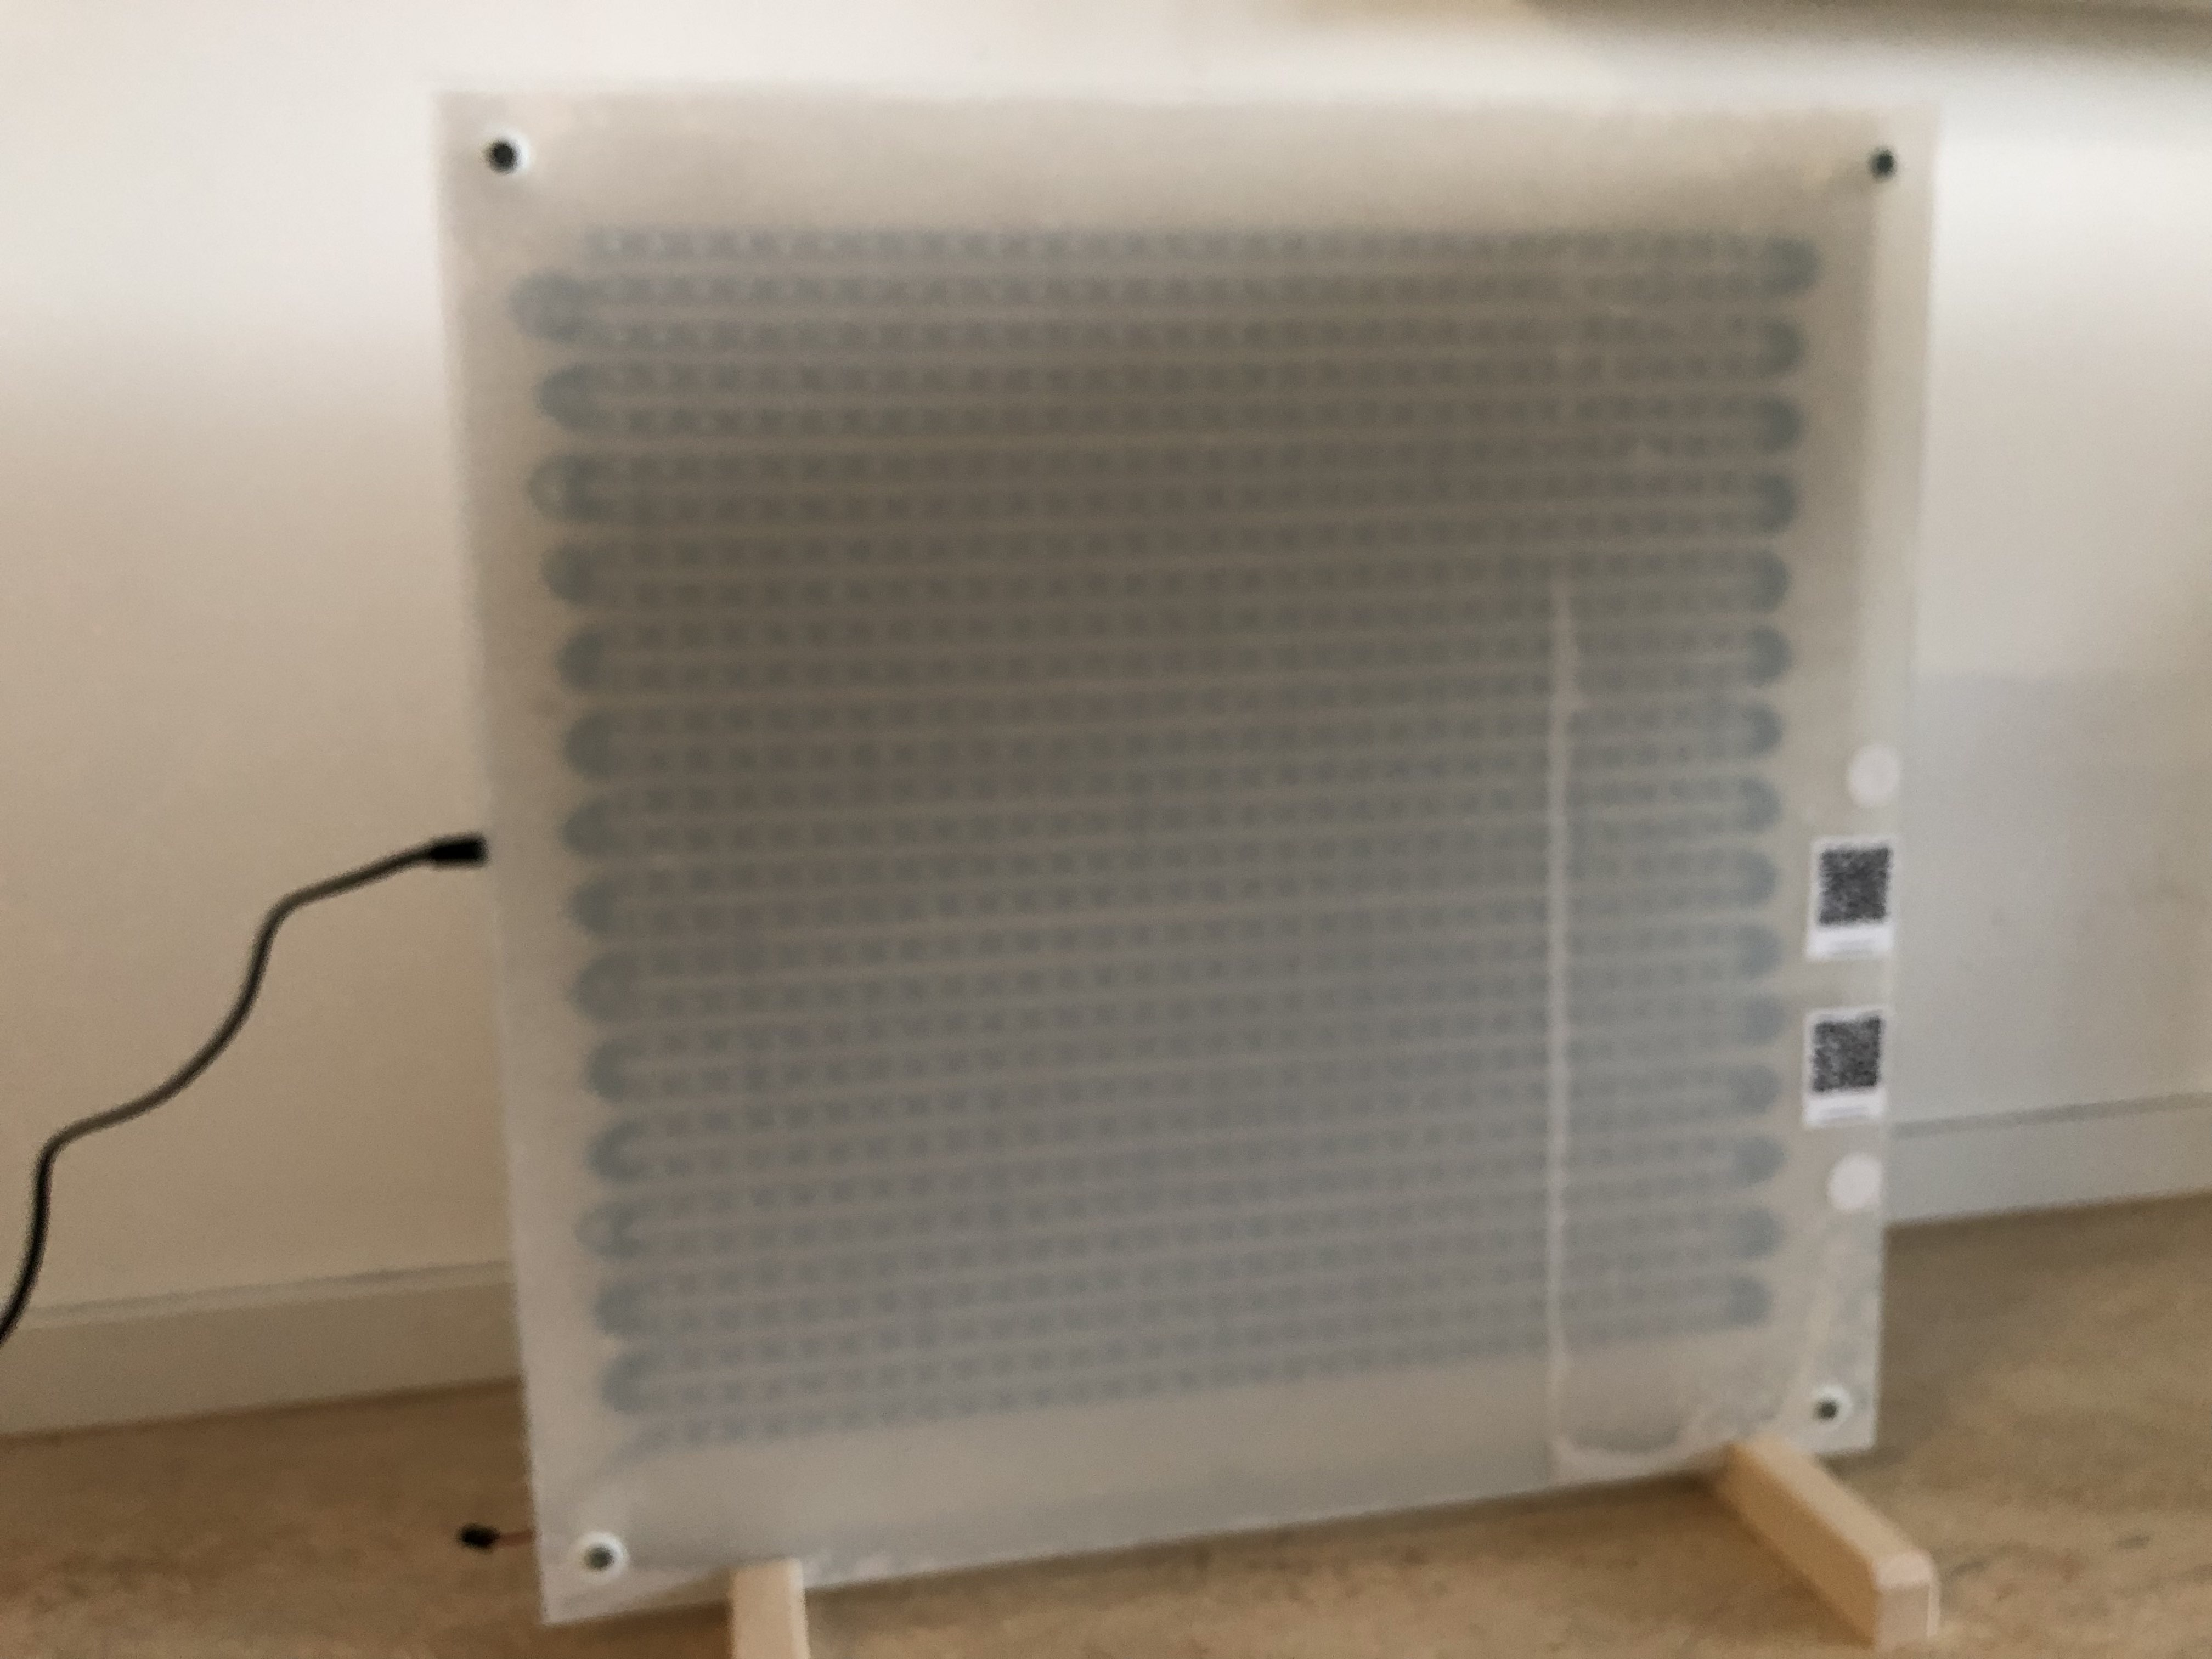
\includegraphics[scale=0.07]{LEDBoard.jpg}
	\caption{Foto des Boards}
	\label{fig:LED-Board}
	\end{figure}

\subsection{Ziele und Erwartungen}
Das Vorgängerteam hat eine gute Arbeit geleistet. Unsere Aufgabe ist es, die Schwächen des Vorgängerprojektes auszugleichen und eigene Verbesserungen/Ideen zu integrieren. Unser Augenmerk liegt auf einer gut ausgearbeiteten, stabilen und sicheren Verbindung vom Endgerät mit dem LED-Board. Das Webinterface muss benutzerfreundlich, intuitiv und unabhängig vom Betriebssystem des jeweiligen Gerätes nutzbar sein. 
Es ergeben sich folgende Ziele: 

\begin{itemize}
\item Auf dem LED-Board sollen grafisch reduzierte Spiele gespielt werden können, wie zum Beispiel  \glqq {Snake}\grqq,\glqq {Tetris}\grqq{} oder \glqq {Pong}\grqq.
\item Die Hardware wird mit einem Microcontroller gesteuert, welcher zusätzlich ein lokales Netzwerk aufsetzt.
\item Spieler sollen in der Lage sein, sich in dieses Netzwerk mit ihren privaten Mobilgeräten zu verbinden.
\item Vom Microcontroller wird eine Webanwendung gehostet, welche als Steuerungseinheit dient.
\item Von der Webanwendung aus können gewählte Spiele gestartet werden und auch ein Mehrspielermodus wird verfügbar sein.
\end{itemize}
     
Hinzu kommen folgende Erwartungen an das Modul: 
\begin{itemize}
\item Vertiefen des gesamten Soft-/Hardware Entstehungsprozesses
\item On-Hand Erfahrung im Team 
\item Vertiefung des Verständnisses von Embeddedprojekten
\item Vertiefung der Programmierkenntnisse
\end{itemize}

Da die Projektaufgabe im teamorientierten Ansatz gelöst werden soll, können hier Soft Skills trainiert und erprobt werden, die zur Koordination von Arbeitspaketen hilfreich und notwendig sind, wie zum Beispiel Teamfähigkeit, Kommunikationsfähigkeit, Selbstorganisation, Projektorganisation, Projektmanagement, Verlässlichkeit und Kritikfähigkeit.

%Enter Text here end

%------------------------------------------------------------------
%Kapitel 2 - Allgemeines
%------------------------------------------------------------------

\section{Allgemeine Informationen}
In diesem Kapitel soll ein Einblick in die Teamstruktur und die Voraussetzungen, auf deren Basis das Projekt entwickelt wurde, gegeben werden. Die Beschreibung der technischen Hilfsmittel und verwendeten Tools soll einen tieferen Einblick in die Arbeitsweise unserer Gruppe vermitteln.

\subsection{Teamvorstellung}
Unsere Gruppe besteht aus vier Teammitgliedern, Lukas Landgraf, Reilly Ertman, Khan Ali Muttaqy und Lisa-Marie Dengler. Wir befinden uns alle im sechsten Semester der Technische Informatik (IT6). Alle Mitglieder der Gruppe verfügen über Kenntnisse der vorangehenden Semester und eigens vertiefte praktische Fähigkeiten, welche insgesamt das Team gut vervollständigen. 

\subsection{Aufgabenbereiche und Arbeitsteilung}
Für verbesserte Effektivität und Zusammenarbeit an diesem Projekt, haben wir uns dazu entschieden, die Umsetzung in Aufgabenbereiche aufzuteilen. 
\begin{itemize}
\item Reilly Hardwareansteuerung, LEDs und Hardware/Software Schnittstelle
\item Khan - Hardwareansteuerung und LEDs
\item Lukas - Backend, Schnittstellenkommunikation und ReversiXT
\item Lisa-Marie - Frontend, Snake und Gruppenorganisation 
\end{itemize}

\subsection{Technische Spezifikationen}
In diesem Projekt werden die Programmiersprachen C/C++ \hspace{0.5ex}unter dem Standard C++20 verwendet.
Der Grund dafür liegt im Erfahrungswert und Kenntnisstand bezüglich dieser Programmiersprache, da alle Gruppenmitglieder mit \hspace{0.5ex}am besten vertraut sind. \\
C++20 ist auch der aktuellste Standard, der zur Verfügung steht. Dadurch wird ein größtmöglicher Umfang an Funktionalitäten durch Programmbibliotheken bereitgestellt.
\vspace{1ex}\\
Das Hostbetriebssystem aller verwendeten Rechner ist Windows 10/11, 64 Bit.
\vspace{1ex}\\
Die verwendete IDE ist \textit{Visual Studio Code} (V 1.78.0 user setup). 
\vspace{1ex}\\
Bei dem verwendeten Microkontroller handelt es sich um einen \textit{ESP32 Wroom-32u}. Dieser ist in der Lage ein eigenes Netzwerk zu hosten und verfügt über ausreichend Speicherplatz für die Webseite, Netzwerkhosting, die Schnittstellen und die Logik der Spiele. 
\vspace{1ex}\\
Um die Umsetzung des Projektes möglichst gut zu bewerkstelligen, verwenden wir die folgenden Tools: 
\begin{itemize}
\item Zum Kompilieren der Quellcodes benutzen wir \textit{Cmake} Version: 3.16
\item In Visual Studio Code verwenden wir die \textit{PlatformIO} Erweiterung
\item Abgestimmt auf PlatformIO verwenden wir das Framework \textit{ESP-IDF}. 
\item Das Frontend der Webanwendung verwendet HTML, CSS und Javascript. 
\item Verschiedene Bibliotheken zum Ansteuern der LED's. 
\item Für Versionskontrolle und gemeinsames Arbeiten nutzen wir \textit{GitLab}
\item Zur Kommunikation innerhalb der Gruppe verwenden wir \textit{Discord}.
\item Erstellung des Projektberichts mit TEXMaker Version: 5.1.3 
\end{itemize}

\newpage

%------------------------------------------------------------------
%Kapitel 3 - Vorab
%------------------------------------------------------------------

\section{Vorüberlegungen und Entwurfsphase}
%Enter Text here start, If you want a new line add -> \\ behind. 
%Anführungszeichen = glqq deinWortgrqq{}
\subsection{Vorüberlegungen (Reilly) } 
Wir setzen das Projekt von Studierenden aus letztem Semester fort. Um zu spielen musste man ein App herunterladen und dies verwenden als Spielcontroller. Dann verbindet man das Handy mit dem Mikrocontroller über Bluetooth. Das Spielen über Bluetooth hat sich als unstabil und unzuverlässig bewiesen. Immer wieder war die Verbindung weg. Auch die Ansteuerung über ein App ist nicht ideal, denn Apps sind dadruch HandyHersteller- und Handyversion abhängig. Das App aus der Gruppe vom letzten Semester muss immer wieder überprüft und ggf. gewartet werden, wenn ein neue Handyversion veröffentlicht wird. 
\vspace{1ex}\\
Deswegen haben wir ein Mikrokontroller aufgesucht, das sowohl ein eigenes WLAN Netzwerk als auch eine Webseite hostet. Spielansteuerung über eine Webseite ist Handyhersteller- und Handyversion unabhängig, was die Wartungskosten deutlich sinkt. Um zu spielen muss man nur zwei QR Codes scannen um loszulegen, eines um zur WLAN zu verbinden und ein zweites um die Webseite aufzurufen. 
\vspace{1ex}\\
Ein integrietes WLAN und gehostete Webseite die vorallem gleichzeitig laufen bedeutet viel Rechenlast. Wenn parallel ein Spiel und noch 900 LEDs gesteuert werden soll, muss das gewählte Mikrokontroller zwingend merhkernig sein.
\vspace{1ex}\\
Da die 900 ws2812b LEDs asynchron und seriel verbunden sind, waren die Auswahl an Kommunikationsprotokolle eingeschränkt. Die LEDs besitzen keinen Ausgang um ein ACK zu senden, also ist I2C nicht möglich. Außerdem haben die LEDs spezielle Timing-Anforderungen (mehr dazu im Kapitel Implementierung). Um Bit Information als Farbe und Helligkeit zu dekodieren müssen die LEDs ständig und immer in der gleichen Geschwindigkeit Information vom Mikrokontroller fangen. Als Protokoll eignet sich UART auch nicht: Es gibt keine Baudrate mit einer Fehlerquote unter 1 Prozent in der Geschwindigkeit, die die LEDs brauchen um Bit Information in Farbe und Helligkeit zu dekodieren. Es bleibt also wenige asynchrone, serielle Protokolle übrig. Am besten wäre ein eingebettenes Waveform-Generator, womit wir direkt mit den LEDs kommunizieren könnten. Dafür biete das ESP32 das RMT Peripheral an (mehr dazu in Implementierung). 
\subsection{Vorüberlegungen }

\subsection{Konzept (Reilly)}
Unser Ziel war es die Zeit und der Aufwand ein Spiel zu starten und zu zocken möglischt kurz zu halten, sonst ist die Motivation zum Zocken weg bevor das Spiel begonnen hat. Man steckt das Board an, verbindet sich mit dem Netztwerk, ruft die Webseite auf, wählt das Spiel aus dem Menü aus und Voilà! Schon ist man am Zocken.

\subsection{Konzept}

\subsection{Design und Architektur (Lukas)}
%Enter Text here start, If you want a new line add -> \\ behind. 
%Anführungszeichen = glqq deinWortgrqq{}
Das Softwaredesign soll es ermöglichen, Spiele ohne große Verzögerung zu starten, zu spielen und zu beenden, sodass das ganze Gerät nicht neugestartet werden muss. Gleichzeitig können Spiele nachträglich hinzugefügt werden, ohne etwas an der Implementierung der LED Steuerung oder dem Webserver ändern zu müssen. Es muss zudem möglich sein, dass alle Teammitglieder möglichst parallel arbeiten können und nicht auf andere warten müssen.
\vspace{1ex}\\
Aus diesem Grund kann unser Design in vier Blöcke unterteilt werden (siehe Abbildung \ref{fig:Architektur}):
\begin{itemize}
\item das Backend, welches das Netzwerk, den Webserver und das Steuern von Spielen implementiert
\item die LED Board Steuerung, die eine simple Schnittstelle für den Spieleentwickler liefern soll, um das Board ohne Schwierigkeiten steuern zu können
\item die Website, welche mit dem Backend für die Spielesteuerung kommuniziert
\item die Spiele selber, die all diese Schnittstellen nutzen
\end{itemize} 
\begin{figure}[h]
\centering
\includegraphics[width=0.75\linewidth]{Architektur}
\caption{\label{fig:Architektur}Darstellung der unterschiedlichen Blöcke und deren Schnittstelleninteraktion in unserer Implementierung.}
\end{figure}

Da diese Blöcke parallel arbeiten müssen, um schnelle Spielsteuerung zu gewährleisten, wird hierfür ein Real Time Operating System benötigt, welches es ermöglicht, die einzelnen Aufgaben auf Tasks aufzuteilen. Hierfür haben wir uns für das ESP-IDF entschieden, das ein Framework für die Entwicklung auf ESP Mikrokontrollern ist \cite{ESSPRESSIF:Reference}. Mithilfe von FreeRTOS, welches in ESP-IDF enthalten ist \cite{ESSPRESSIF:Reference}, können die einzelnen Blöcke, wie Webserver und Spiele, auf eigenen Tasks laufen. Zusätzlich bietet ESP-IDF auch eine Menge nützlicher APIs für z.B. Webserver oder die Bedienung der Pins an \cite{ESSPRESSIF:Reference}.
\vspace{1ex}\\
\newpage

%------------------------------------------------------------------
%Kapitel 4 - Implementierung
%------------------------------------------------------------------

\section{Implementierung}
%Enter Text here start, If you want a new line add -> \\ behind. 
%Anführungszeichen = glqq deinWortgrqq{}

\subsection{LED-Ansteuerung und Hardware (Reilly)} 
Am GPIO des ESP32 muss eine Spannung erzeugt werden. Diese elektrische Spannung fließt dann durch eine Leitung an den Eingang des ersten asynchronen ws2812b LED in der Kette. Die Spannungen müssen bis zu einer Granularität von 50ns einstellbar sein. Die Erzeugung der Spannung soll so rechnenschonnend sein wie möglich. Die LEDs müssen dieses Protokoll verstehen.
\vspace{1ex}\\
Hierfür biete das ESP32 das RMT (Remote Control Transceiver) Peripheral an. Da dieses eingebettene Waveform-Generator Signale alle 10ns erzeugt und Direct Memory Access (DMA) benutzt, was der Last an das CPU deutlich verringert, haben wir uns für das RMT Peripheral entschieden.
\vspace{1ex}\\
\subsubsection{WS2812B LED Protokol}
Ein ws2812b LED besitzt folgedes Interface: ein einziges Data\textunderscore in, Masse und VCC. Pro LED werden 24 bit Information benötigt um das LED zu beleuchten. Die 3 byte eines LED Array besteht aus 3 Teilen: Ein byte für das Grüne, das Rote und das Blaue Anteil jeweils. Umso hörer die jeweilige Byte-Werte, desto heller leuchtet das LED. Um das LED Grün zu beleuchten, setzt man das erste Byte auf 0, das zweite auf 255 und das letzte Byte auf 0. Um Weiß auszugeben, lauten die Byte-Werte 255/255/255.
\vspace{1ex}\\
Da wir nur ein einzelnes Data\textunderscore in am Interface zur Verfügung haben, ist der Data\textunderscore out vom ersten LED das Data\textunderscore in vom zweiten LED, usw. Die ws2812B Kette bildet also ein Daisy Chain. Um das letzte von 900 LEDs in der Kette anzuleuchten, müssen diese Daten erst durch alle 899 LEDs durchgeschoben werden. Genau müssen diese bits 21600 Bitstellen (3 byte * 900 * 8) passieren. Dieses Verfahren heißt "Bit Banging". Man stelle sich vor jedes ws2812b wäre ein Schieberegister mit 24 bit jeweils. Wenn das erste Bit in der Leitung das Least Significant Bit des letzten LEDs in der Kette erreicht, sind die Daten dann an der richtigen Stelle.

	\begin{figure}[h]
	\centering
	\includegraphics[width=1\linewidth]{ws2812b-1}
	\caption{\label{fig:Oscillosope}WS2812b liest eingehend Spannungen bzw. Wörter an der Leitung.}
	\end{figure}

Abbildung 3 zeigt eine Oscillosope Ausgabe eines Datenpakets. CH1 beinhaltet 48 bit binäre Information am Eingang des ersten LEDs und CH2 ist der Signal am Ausgang gemessen. Beide Signale beinhalten mehrere steigende und fallende Flanken. Die dargestellten analogen Signale sind vom Mikrocontroller erzeugt mit spezifischen Timing Anforderungen; nämlich, die Kombination aus einer steigenden und fallenden Flanke bildet ein Wort. Dieses vom Mikrokontroller enkodiertes analoges Signal wird dann vom WS2812b als Wort dekodiert und bildet entweder ein Logical 1 oder 0. Kommt 24 solche Signale, können wir ein einzelnes LED anleuchten.
\vspace{1ex}\\
In dem Beispiel aus Abbildung 3 werden eine Reihe an Spannungen an das WS2812b geschickt. Konkret wird das folgende Wort zwei mal hintereinander dekodiert: 100101100000000000000000. Die ersten 8 bit "10010110" beinhalten die Helligkeit für das Grüneanteil des LEDs. Rot und Blau haben den Wert 0. Weil das Wort zwei mal hintereinander steht, werden am Ende 2 LEDs Grün leuchten. Danach wird die Leitung auf 0 gezogen. Wenn 0 konstant nach einer Übertragung ausgegeben wird, kommt keine weiter Information und die LEDs sollen ihren letzten Zustand behalten. \cite{esptiming:Doku}
\vspace{1ex}\\
WS2812B Timings: Jedes bit ist also vom ESP32 enkodiert als ein Pulsweitenmodulationssignal mit einem gewissen Duty Cycle. Das Datenblatt vom Hersteller erläutet genauer über die Timing der Pulsweitenmodulation in Abbildung 4 und 5. \cite{esptime32:Dok}

	\begin{figure}[h]
	\centering
	\includegraphics[width=0.5\linewidth]{ws2812b-2}
	\caption{\label{fig:logic}Ein ws2812b Wort besteht aus einem high gefolgt von 		einem low Part.}
	\end{figure}
	\begin{figure}[h]
	\centering
	\includegraphics[width=0.8\linewidth]{ws2812b-3}
	\caption{\label{fig:timing}WS2812b Die Länge eines Wortes in Nanosekunden.}
	\end{figure}
	
Sollte ein LED Grün leuchten, müssen die ersten 8 von 24 bits auf '1' gesetzt sein und der Rest auf '0'. Für jedes gesetzes Bit muss am Output Pin des ESP32 ein "high" Signal für 0,8us gefolgt von einem "low" Signal für 0,45us ausgegeben werden. Die Kombination aus T1H und T1L versteht ein WS2812B LED als ein Logical 1. Soll ein Bit nicht gesetzt werden, erzeugt das ESP32 am Output Pin ein "high" Pegal für 0,4us gefolgt von einem "low" Pegal für 0,85us. Daraus versteht das ws2812b das Signal als ein logical 0. Wenn für mindestens 50us lang am Dataline 0V Signal anlegt, behalten die LEDs ihren Zustand. \cite{esptime32:Dok}
\vspace{1ex}\\
\subsubsection{Bitübertragunsschicht des ESP32 und das RMT Peripheral}
Wenn man Daten an ein WS2812b LED senden möchte, gibt es ein Problem. Das WS2812b Protokol ist asynchron und bietet keine Möglichkeit von einem Hardware Handshake gebrauch zu machen. Das heißt wir müssen den größten gemeinsamen Teiler von T0H, T1H, T0L und T1L nehmen als Taktfrequenz, also 50 ns. Das ist nun die Granularität, mit dem wir die benötigten steigenden und fallenden Flanken bilden können, um mit dem Ws2812b kommunizieren zu können.
Um Signale alle 50ns auszugeben, bietet das Esp32 einen eingebetteten und schlichten Waveform Generator an: das Remote Control Transceiver, genannt als RMT. 
\vspace{1ex}\\
Das ESP32RMTChannel.h Headfile kümmert sich um die Erstellung des RMT-Modules als Transceiver. Die Funktion ConfigureForWS2812x() instanziiert das RMT am gewünschten GPIO und mit gewünschten Prescaler. Da das Clock der RMT bei 80MHz liegt, wählen wir einen Prescaler von 4 aus um eine Taktfrequenz von 20MHz bzw. 50ns zu erreichen. 
\vspace{1ex}\\
Das ESP32 biete zwei legacy libraries, die wir zur Instanziierung und Verwendung des RMTs benötigen: rmt\textunderscore config\textunderscore t und rmt\textunderscore types \textunderscore legacy. rmt\textunderscore legacy.c biete die Funktion rmt\textunderscore write\textunderscore items() und erzeugt die gewünschten getaktete Spannung am GPIO. Wie bereits besprochen passieren auf dem data\textunderscore in des LED Boards eine Reihe von steigenden und fallenden Flanken, wohingegen der Programmierer ist dafür zuständig die gewünschten Bits in den Buffer zu schaffen, die das LED Board anleuchten soll. Aber was passiet dazwischen und wie werden die digitale 1s and 0s auf dem Bildschirm zu getakteten Spannung am GPIO übersetzt? Dies erledigt der Datatype rmt\textunderscore item32\textunderscore t aus rmt\textunderscore types\textunderscore legacy.h für uns. \cite{esptime32:Dok}

	\begin{figure}[h]
	\centering
	\includegraphics[width=0.8\linewidth]{ws2812b-4}
	\caption{\label{fig:timing}WS2812b reads timed high and low voltages and 1s and 	0s.}
	\end{figure}
	
rmt\textunderscore item32 \textunderscore t ist ein 32-Bit integer union struct bestehend aus 4 Elementen in chronlogischer Reinfolge: duration0, level0, duration1,level1. Ein Union Struct heißt alle Mitglieder teilen den gemeinsamen Datenbereich. Die Bitbelegung der Mitglieder laut Abbildung 5 sieht aus wie gefolgt:

\begin{itemize}
\item rmt\textunderscore item32 \textunderscore t(31 downto 17) = duration0
\item rmt\textunderscore item32 \textunderscore t(16) = level0
\item rmt\textunderscore item32 \textunderscore t(15 downto 1) = duration1
\item rmt\textunderscore item32 \textunderscore t(0) = level1
\end{itemize}

Um ein T0H auszugeben, setzen wir Duration0 auf den in DLEDController schon ausgerechneten Wert und level0 auf high. Um T0L auszugeben, setzen wir Duration1 auf den entsprechenden Wert und dann level1 auf 0. T0H + T0L wird am Esp32 GPIO dann als ein Logical 0 vom ws2812b verstanden. 

\subsubsection{LED Benutzeroberfläche}
Ein LED Brett wird als Objekt der Klasse DStripData instanziert. Das Brett-Objekt besitzt ein 3D Array von 3*NUM\textunderscore OF\textunderscore LEDS uint8 \textunderscore t. Wenn der C/C++ Compiler ein x-D Array in Speicher kompiliert, wird Speicher mit einem Uni-Dimensionales Array beschrieben. Daten des kleinsten Indizes werden zusammenhängend geschrieben, wie gefolt:
	
	\begin{verbatim}
	Array[2][5][3] = Array_1[5][3], Array_2[5][3];
	Array_1[5][3]={{0,1,2},{3,4,5},{6,7,8},{9,10,11},{12,13,14}};
	Array_2[5][3]={{15,16,17},{18,19,20},{21,22,23},{24,25,26},{27,28,29}};
	Array[2][5][3] = | 0 | 1 | 2 | 3 | 4 | 5 | 6 | 7 | 8 | 9 | 10..
	..| 11 | 12 | 14 | 15 | 16 .. | 29;
	\end{verbatim}

Dieses Schema muss man im Kopf behalten, denn wenn alle 900 LEDs bei 20Hz aktualisiert werden, soll man das Array lieber via Pointerarithmetik traveriseren um Performance zu maximieren. Ansonsten schafft das CPU die Daten nicht schnell genug. 
\vspace{1ex}\\
Zum Spieleschreiben bietet sich Objektorientiertes Programmieren hervorrangend an. Wird bei Snake ein Pixel von der Schlange gefressen, wird das Pixel Objekt zerstört und dabei z.B. ein Event ausgelöst. Deswegen steht Pixel.h zur Verfügung.
\vspace{1ex}\\
Als Programmieren gibt es also zwei Möglichkeiten das LED Brett zu beschreiben: (1) Durch direktes schreiben des 3D Arrays oder (2) das objektorientiertes Programmieren in dem man Objekt erzeugt und dies mit anderen Objekt interagiert.
\subsubsection{Kritischer Bereich und Double Buffering}
Ist das 3D Array vollständig beschrieben mit Pixeldaten, dann wird der Vorgang gestartet, endlich ein Bild auf das LED Brett zu bringen. Dafür muss das RMT Peripheral das 3D Array nun ablesen und in elektrischen Spannungen übersetzen. In dieser Zeit darf das 3D Array nicht beschrieben werden. Hat das RMT Peripheral das 3D Array fertig gelesen, wird das Array freigeben und kann wieder beschrieben werden.
\vspace{1ex}\\
Um ein flüssiges Spiel für das menschliche Auge zu gewährlisten, ist ein minimales Frame Rate notwendig. Die Übertragung eines Bits (die Zusammensetzung von T0H+T0L oder T1H+T1L) dauert ungefährt 1,2us. Bei 21600 Bits insgesamt, rechnet sich ein ideales Frame Rate von 33Hz aus. Da das CPU aber verschiedene Programme (Wifi, Webseite, Spiele, usw.) gleichzeitig jongliert, liegt das Frame Rate bei ca. 15 Bilder pro Sekunde. Für ein 1920 x 1080 PC Monitor mit über 2.000.000 Pixeln wären 15 Bilder pro Sekunde sofort bemerkbar. Wenn der Monitor jedoch nur 900 Pixel hat, ist der Vorteil eines flüssigeren Spiels angesichts der hohen Kosten für die CPU-Leistung marginal. Bei 900 Pixeln merkt man keinen Unterschied zwischen einer Bildrate von 30 oder 15.  
\vspace{1ex}\\
Der Programmier darf nicht zu beliebeigen Zeiten das LED Brett beschreiben. Das ist nur erlaubt zu der freigegebenen Zeit. Um die erlaubte Zeit des schreibens maximal groß zu halten wird double buffering eingesetzt. So bleibt der kritischer Bereich minimal klein, in dem man das LED Board nicht beschreiben darf. Bei einer Bildwiederholungsrate von 15Hz wird alle 70ms ein neues Bild erstellt und angezeigt. Bevor ein Bild angezeigt wird, muss es beschrieben werden. Es gibt also zwei Phasen zur Erstellung eines Frames: Das Beschreiben des Bildes, wo das schreiben erlaubt ist, und Anzeigen des Bildes, wo das schreiben nicht erlaubt ist. Würde beide Phasen über einem Buffer ablaufen, dürfte man nur die Hälfte der Zeit (35ms) das Bild beschreiben, denn in der Zeit wo das Bild angezeigt wird dürfte es nicht angefasst werden. Mit Double Buffering allerdings wird nach jede ca. 35ms das neulich beschriebenes Bild kopiert. Das Anzeigen läuft dann über die Kopie, bzw., über das zweite Buffer. So wird einem das Schreiben eines Bildes praktisch nie gesperrt wird. 
\vspace{1ex}\\
Diese Strategie kann man allerdings nur einsetzen, wenn der benötigte Speicherplatz vorhanden ist. Die Channelbuffer attribute in RMT.cpp hat eine größe von (900 LEDs * 3 Byte in einem LED * 8 bit * 32bit pro RMT\textunderscore item) 86 KB. Laut Datenblatt wird das SRAM in drei Kategorien unterteilt. Die kleinste davon hat 120 KB Speicher, Um diese Variable runterzubekommen auf mein SRAM muss ich ins Datenblatt schauen.

\subsubsection{Flackernde Frames (Lukas)}
Während der Nutzung von Arcade LED ist oftmals ein Flackern von mehreren LEDs in verschiedenen Farben auf dem Board für einen Frame sichtbar (siehe Abbildung \ref{fig:Flackern}). Dieses Flackern ist erst entstanden, nachdem die LED Board Steuerung mit dem Webserver und Spieletask gleichzeitig verwendet wurde. Somit ist uns dieses Problem erst sehr spät während der Spieleentwicklung aufgefallen.
 \begin{figure}[h]
\centering
\includegraphics[width=0.5\linewidth]{Flackern}
\caption{\label{fig:Flackern}Ein von Flackern betroffener Frame des Spiels Snake}
\end{figure}
\vspace{1ex}\\
Zuerst wurde überprüft, ob der Spieletask selbst dem Senden durch z.B. zu frühes Aufrufen von rmt\_write\_items() in die Quere kommt. Allerdings ist dies nicht der Fall, da nach jedem Aufruf der Funktion ein Delay eingebaut ist. Außerdem kann der Funktion ein Flag übergeben werden, durch das erst nach dem vollständigen Senden aus dieser zurückgekehrt wird\cite{ESSPRESSIF:Reference}. In beiden Fällen hat sich nichts am Flackern verändert.
\vspace{1ex}\\
Da der einzige Task, der auf die DLEDControllerklasse zugreift, der Spieletask ist und somit nur dieser allein Daten auf das Board sendet, müssen es die anderen Tasks sein, die dem Senden in die Quere kommen.  Durch Testen haben wir herausgefunden, dass das Flackern entsteht, wenn während der Übertragung auf das Board eine Nachricht auf dem Webserver oder Netzwerk eintrifft. Besonders starkes Flackern ist sichtbar, falls eine Website geladen wird.
\vspace{1ex}\\ 
Wie in folgenden Kapiteln genauer beschrieben wird, wurde der Spieletask auf Kern 1 und alle anderen Tasks, wie der Webserver, auf Kern 0 gemappt. Somit sollten sich die beiden nicht in die Quere kommen. Dies hat allerdings für keine Veränderung am Flackern gesorgt.
\vspace{1ex}\\ 
Auf dem ESSPRESSIF ESP-IDF Forum gibt es einen Post mit dem genau gleichen Problem. Ein ESP soll eine Reihe an WS2812 LEDs über einen SPIFFSbasierten Webserver ansteuern. Sendet der Webserver eine Datei an einen Client, ist ein Flackern auf den LEDs zu sehen \cite{ESSPRESSIF:Forumspost}. Die angegebene Lösung für das Problem ist es, das \dq ESP\_INTR\_FLAG\_IRAM\dq{} Flag bei der Installation des RMT Drivers anzugeben \cite{ESSPRESSIF:Forumspost}. Dieses sorgt dafür, dass die Interrupt Service Routine, die für das Senden des Signals zuständig ist, permanent im Instruction RAM ist \cite{ESSPRESSIF:Reference}. Wäre dies nicht der Fall, müsste möglicherweise die ISR erst aus dem Flash geladen werden \cite{ESSPRESSIF:Reference}. Falls in diesem Moment der Flash allerdings durch das Laden einer Website besetzt ist, könnte dies zu Problemen führen. Für unsere Implementierung hat dies das starke Flackern beim Aufrufen einer Website verringert, aber nicht entfernt.\vspace{1ex}\\ 
Mithilfe von Semaphoren wurde sichergestellt, dass das Senden an das Board und Bearbeiten der Requests an den Webserver nicht gleichzeitig stattfinden kann. Dies hat das Flackern vollständig entfernt, aber auch für enorme Ladezeiten auf der Website gesorgt und die Spielsteuerung gestört. Zudem hat es während des Sendens einer Seite zu Standbildern auf dem LED Board gesorgt. Aus diesen Gründen wurde die Semaphoren wieder entfernt.
\vspace{1ex}\\ 
Trotz Ausprobierens vieler verschiedener Lösungen konnte keine akzeptable für dieses Problem gefunden werden, weswegen immer noch Flackern auf dem LED Board erscheint.
\subsection{Backend   (Lukas)} 
\subsubsection{Netzwerk}
Mithilfe der ESP-IDF API ist es möglich, auf ESP-WROOM Boards das Wi-Fi Modul zu nutzen, um sich mit Netzwerken zu verbinden oder eigene zu erstellen \cite{ESSPRESSIF:Reference}. Für Arcade LED haben wir uns dazu entschieden, ein eigenes Netzwerk auf dem ESP zu verwenden. Somit ist man nicht auf extra Geräte, wie Router, angewiesen, sondern benötigt nur den ESP, das LED Board und eine Stromversorgung.
\vspace{1ex}\\
Die Erstellung des Netzwerks geschieht beim Starten des Systems, bevor die einzelnen Tasks aufgerufen werden. Hier wird auch mithilfe von mehreren API Funktionen das Netzwerk konfiguriert. In unserem Fall wurden bis auf die Kernzuweisung und kleinere Konfigurationen, wie den Namen, die Standardeinstellungen übernommen. Durch die Kernzuweisung auf Kern 0 der zwei Kerne des ESP wurde sichergestellt, dass das Netzwerk dem Spieletask, der auf Kern 1 läuft und eventuell ein neues Bild an das Board sendet, nicht in die Quere kommt.
\vspace{1ex}\\
Die Verbindung mit dem Netzwerk ist stabil und selbst mit vier Spielern gleichzeitig schnell genug. Allerdings gab es während der Entwicklung auch Schwierigkeiten. Zu Beginn des Projekts bestanden starke Verbindungsprobleme, die Reichweite und die Stabilität des Signals waren sehr schlecht. Die Ursache hierfür war eine fehlende Antenne auf den ESP-32WROOM-32D Boards \cite{ESP:Datasheet}, die verwendet wurden. Mithilfe einer externen Antenne und später des ESP-32WROOM-32U Boards, welches eine interne Antenne besitzt \cite{ESP:Datasheet}, konnte eine sichere Verbindung hergestellt werden.
\vspace{1ex}\\
Ein weiteres Problem, welches allerdings nicht gelöst werden konnte, ist ein Fehler bei der IP Adressenvergebung. Falls, während ein Gerät mit dem Netzwerk verbunden ist, ein Neustart durchgeführt wird und anschließend nach dem Neustart ein weiteres Gerät sich verbindet, kann es dieselbe Adresse wie das erste Gerät erhalten. Gerät 1 hat allerdings nie den Neustart bemerkt und somit denkt es, die IP Adresse ist noch gültig, kann aber keine Nachrichten mehr empfangen. Da das Problem nur manchmal bei Neustarts auftritt und laut Internetquellen es keine andere Lösung gibt, außer zu warten, bekam dieser Bug eine niedrige Priorität.

\subsubsection{Webserver}
Um eine einfache Spielsteuerung auf allen Geräten zu ermöglichen, haben wir uns für eine Website entschieden. Diese Website wird auf dem ESP mithilfe der Webserver API der ESP-IDF gehostet. Die API ermöglicht es, selbstgeschriebene Funktionen auf HTTP Requests und URLs zu registrieren \cite{ESSPRESSIF:Reference}. Die Funktionen werden aufgerufen, falls der korrekte HTTP Request mit URL eintrifft.
\vspace{1ex}\\
Wenn man in einem Browser eine URL eingibt, wird von diesem ein HTTP Get Request mit der URL als Inhalt an den Webserver gesendet. Solange dieser Request mit der URL \dq/Webapp\dq{}  beginnt, wird auf unserem Webserver eine Funktion aufgerufen, die aus der URL den Dateipfad ausliest, die korrekte Datei öffnet und diese als Antwort an den Browser zurücksendet.
\vspace{1ex}\\
Die Dateien der Website sind auf dem Flash des ESPs auf einer zweiten Partition mit einem SPIFFS Dateisystem gespeichert. ESP-IDF bietet auch hier APIs an, um solche Dateisysteme zu erstellen und zu verwenden \cite{ESSPRESSIF:Reference}. Dies kommt allerdings mit einigen Limitierungen. Dateinamen sind auf 32 Zeichen beschränkt \cite{ESSPRESSIF:Reference}. Zusätzlich ist dieses Limit schnell erreicht, weil es keine Ordner gibt und diese stattdessen zum Dateinamen hinzugefügt werden \cite{ESSPRESSIF:Reference}. Da ESP32 Code, der nicht explizit im IRAM gespeichert wurde, vor der Ausführung erst vom Flash geladen werden muss, kann es eventuell für Interrupt Service Routinen zu Problemen führen, wenn eine sehr große Datei gesendet wird, in diesem Moment aber die ISR nicht im IRAM ist \cite{ESSPRESSIF:Reference}.
\vspace{1ex}\\
Ein weiterer Request Handler reagiert auf die URL  \dq/Data\dq{}. Dieser ist dazu gedacht, Daten über den Zustand der Lobby und der Spieler als Antwort zurückzusenden (siehe Abbildung \ref{fig:Data}). Somit ist es möglich, auf der Website anzuzeigen, ob bereits ein Spiel läuft oder wie viele Spieler noch benötigt werden, um zu starten.
\begin{figure}[h]
\centering
\includegraphics[width=1\linewidth]{Data}
\caption{\label{fig:Data}Die Daten, die auf einen HTTP GET Request auf die URL \dq/Data\dq{} als Antwort zurückgesendet werden.}
\end{figure}
\vspace{1ex}\\
Jedesmal, wenn der Webserver einen Request erhält, wird eine neue Socket für diesen geöffnet. Allerdings wurden alte Sockets nicht nach Versenden der Datei geschlossen und neu eintreffende Requests ignoriert, da nur eine begrenzte Anzahl an Sockets gleichzeitig geöffnet sein kann. Dies sorgte für sehr lange Ladezeiten, falls mehrere Geräte die Website aufrufen.
\vspace{1ex}\\ 
Um dies zu umgehen, gibt es eine Konfiguration im Webserver, welche die am wenigsten zuletzt genutzte Socket schließt \cite{ESSPRESSIF:Reference}. Da dies allerdings auch manchmal die Websockets, welche für die Spielsteuerung zuständig sind, zerstörte, konnte es für unser Projekt nicht verwendet werden. \vspace{1ex}\\
Eigentlich gibt es laut der ESP-IDF Dokumentation eine API Funktion, welche eine Socket nach Vollenden der Aufgabe schließen soll \cite{ESSPRESSIF:Reference}. Da diese allerdings in unserer Version des Frameworks nicht auffindbar war, konnte sie nicht verwendet werden. Stattdessen wird das Error Handling des Webservers ausgenutzt. Falls ein HTTP Request Handler etwas anderes als ESP\_OK zurückgibt, wird es als Error angesehen und die Socket sofort geschlossen \cite{ESSPRESSIF:Reference}. Dies hat keine erkennbaren Verlangsamungen oder negative Folgen für den Webserver und sorgt dafür, dass selbst mehrere Geräte gleichzeitig die Website laden können.



\subsubsection{Spielesteuerung}
Auf Arcade LED ist es möglich, mit bis zu vier Spielern gleichzeitig zu spielen. Jeder dieser Spieler ist in der Lage, mit seinem eigenen Gerät Knöpfe zu drücken, welche eine Nachricht an den Webserver senden. Dieser verarbeitet die Nachricht und ändert den Status des korrespondierenden Knopfes des Spielers. Um festzustellen, welcher Spieler gerade einen Knopf gedrückt hat, müssen allerdings die verbundenen Geräte auf die vier Spielerslots gemappt werden.
\vspace{1ex}\\
Die Übertragung der Nachricht wäre z.B. möglich mit HTTP Post Requests. Um sich zu merken, welcher Spieler die Nachricht gesendet hat, könnte eine SpielerID, welche zuvor vergeben wurde und auf dem Gerät des Nutzers gespeichert wird, als Teil der Nachricht mitgesendet werden. Mit dieser Methode könnte es allerdings möglich sein, dass mehrere Geräte dieselbe SpielerID besitzen. Außerdem kann auf dem ESP nicht überprüft werden, welche Spieler noch verbunden sind. Somit können Verbindungsabbrüche nicht registriert werden.
\vspace{1ex}\\
Websockets hingegen ermöglichen es, eine permanente Verbindung zwischen Webserver und Smartphone zu öffnen \cite{ESSPRESSIF:Reference}. Somit können die SpielerIDs auf die Sockets verteilt werden. Die Verbindung der Spieler kann auch leicht über diese überprüft werden, weil im Falle eines Verbindungsabbruchs die Socket geschlossen wird \cite{ESSPRESSIF:Reference}.
\vspace{1ex}\\
Da die Websockets für die Spielerverwaltung zuständig sind, muss von der Lobbyerstellung bis zum Spielende alles über diese geschehen. Hierfür gibt es drei Befehle.
\begin{figure}[h]
\centering
\includegraphics[width=1\linewidth]{Befehle}
\caption{\label{fig:Befehle}Liste der Befehle, die über die Websocket für die Lobbyerstellung, Lobbybeitreten und Knopfsteuerung gesendet werden können.}
\end{figure}
\vspace{1ex}\\
Der Lobby erstellen Befehl öffnet eine neue Lobby mit dem ausgewählten Spiel und der Spieleranzahl, falls keine Lobby in diesem Moment existiert. Außerdem wird die Websocket, über die dieser Befehl erhalten wurde, als Spieler 1 registriert. Anschließend können andere mit dem Lobby beitreten Befehl ihren eigenen Spielerslot erhalten. Sobald die maximale Spieleranzahl erreicht ist, startet das Spiel und mit dem Knopfdruck Befehl kann der Status des ausgewählten Knopfs auf \dq gedrückt\dq{} oder \dq losgelassen\dq{} geändert werden. Somit ist es möglich, auf der Website auch Knöpfe gedrückt zu halten (siehe Abbildung \ref{fig:Befehle}). 
\vspace{1ex}\\
Wie bereits erwähnt, wird bei Schließung der Websocket der Spielerslot wieder freigegeben und jemand anderes oder die gleiche Person könnte im Falle eines Verbindungsabbruchs wieder beitreten. Sollten allerdings keine Spieler mehr mit der Lobby verbunden sein, wird diese geschlossen und das Spiel beendet. Anschließend könnte erneut eine neue Lobby geöffnet werden. Somit muss der ESP nie neugestartet werden und es ist möglich, ohne Verzögerung weiterzuspielen.



\subsubsection{Spieletask und Taskkommunikation}
Da der Webserver und die Spiele parallel ausgeführt werden müssen, existiert eine extra Task für die Spiele auf Kern 1. Solange kein Spiel gestartet ist, zeigt dieser Task den Startbildschirm auf dem LED Board an. Sobald alle Spieler einer Lobby beigetreten sind, wird anhand der SpieleID die Funktion des korrekten Spiels aufgerufen. Wenn das Spiel beendet werden soll, ist es Aufgabe des Spieleentwicklers, alle dynamischen Objekte, die benötigt wurden, zu zerstören und aus der Funktion zurückzukehren.
\vspace{1ex}\\
Die Kommunikation zwischen Spieletask und Webserver erfolgt über ein Objekt der Lobbyklasse, auf das beide Tasks Zugriff haben (siehe Abbildung \ref{fig:Lobby}). In dieser Klasse werden alle Daten abgespeichert, wie die Knöpfe der Spieler, welches Spiel gestartet werden soll und der Zustand der Lobby. Da es sich hier um einen kritischen Bereich handelt, muss mit Methoden, die mit Semaphoren abgesichert sind, auf diese Variablen zugegriffen werden.
\begin{figure}[h]
\centering
\includegraphics[width=0.85\linewidth]{Lobby}
\caption{\label{fig:Lobby}Das Diagramm zeigt die Kommunikation über die Lobbyklasse zwischen dem Spieletask und dem Webserver.}
\end{figure}
\vspace{1ex}\\
Um ein neues Spiel für Arcade LED zu entwickeln, muss zunächst eine Funktion mit Pointern auf die Lobby und die DLEDController Klasse als Parameter erstellt werden. Die DLEDControllerklasse ist nötig, um das LED Board anzusteuern. In der Funktion kann nun das Spiel entwickelt werden. Es muss allerdings sichergestellt werden, dass regelmäßig der Status der Lobby abgefragt wird, da bei dem Zustand \dq lobby\_closed\dq{} das Spiel beendet werden muss. Sollte das Spiel normal zu Ende kommen, muss die Verbindung aller Spieler mithilfe einer Methode von Lobby getrennt und auch auf eine Veränderung des Lobbyzustands gewartet werden.

\newpage

\subsection{Frontend  (Lisa-Marie)} 
Besonders wichtig für die Entwicklungsrichtung des Projektes war die Entscheidung über eine grafische Benutzeroberfläche. Diese Entscheidung musste sehr früh im Entwicklungsprozess getroffen werden, da die Konstruktion des Backends sehr stark mit der gewählten Oberfläche gekoppelt ist. Die Kommunikation über eine geeignete Schnittstelle muss gut durchdacht sein und die Ansteuerung des LED-Boards ist auf die Grafische Benutzeroberfläche angewiesen, welche die Verbindung zu dem Nutzer darstellt.  

\subsubsection{Vorüberlegungen}
Das Projekt Arcade LED ist die Neuauflage eines früheren Projektes und soll die Schwachstellen der Vorgängergruppe verbessern. Einer der wichtigsten Aspekte des Projektes war die Verbesserung der Kommunikation zwischen den Nutzern und dem LED-Board. Unsere Vorgänger nutzen eine Android App für die Spielauswahl und Steuerung. Leider funktionierte die Steuerung sehr holprig und das Erscheinungsbild/Design der Applikation war sehr kontraintuitiv für die Spieler. 
\vspace{1.5ex}\\
So stellt sich die Frage nach der geeigneten Oberfläche, welche sowohl effektiv in der Kommunikation mit dem Microkontroller als auch einfach in der Benutzung für Spieler ist. Die möglichen Optionen waren auch in unseren Überlegungen entweder eine App oder eine Webseite.
\vspace{1.5ex}\\
%vielleicht lieber ne tabelle mal schauen 
\textbf{Nachteile der App:}\\
\begin{itemize}
\item Plattformabhängigkeit: eine App müsste für die verschiedenen Betriebssysteme separat entwickelt werden und hätte somit einen deutlich höheren Entwicklungsaufwand und potenzielle Kosten. Sich nur auf ein Betriebssystem zu einigen widerspricht unseren Anforderungen für das Projekt. 
\item Installation und Aktualisierung: Diese Apps müssten in den App Stores der jeweiligen Betriebssysteme bereitgestellt und für die Installation verfügbar sein. Bei Anpassungen der Applikation müssten stetige Updates über den App Store ermöglicht werden. Zudem müsste das Endgerät über ausreichend Speicherplatz verfügen. 
\item Kommunikation: Die Schnittstelle der Kommunikation zwischen einer App und einem Microkontroller ist mit unserem ESP32 aufwendiger. Hinzu kommen mögliche Kompatibilitätsprobleme. 
\end{itemize}

\newpage

\textbf{Vorzüge der Webseite:}\\
\begin{itemize}
\item Plattformunabhängigkeit: Eine Webseite kann auf verschiedenen Betriebssystemen und Geräten  genutzt werden, da sie über den Webbrowser zugänglich ist. Dadurch entfällt die Notwendigkeit, separate Versionen für verschiedene Plattformen zu entwickeln.
\item Wartung und Updates: Änderungen an einer Webseite können zentral vorgenommen werden, da sie auf einem Server gehostet wird. Dadurch entfällt die Notwendigkeit, Updates für jede einzelne Installation zu veröffentlichen.
\item Kommunikation: Der Austausch von Daten mit einem ESP32 kann mithilfe einer guten Websocket-Implementierung stattfinden. Für nähere Definition siehe Abschnitt \ref{backend}.
\end{itemize}

Die Wahl zur grafischen Benutzeroberfläche fiel hiermit auf die Webseite, da vor allem in den Anforderungen für unser Projekt keine Festlegung auf ein einziges Betriebssystem gewünscht ist. Die Webseite muss nun in der Lage sein auf den gängigen Wegen via Http erreichbar zu sein. Natürlich muss zusätzlich der grundlegende Zweck zur Steuerung und Spielauswahl erfüllt werden. Die Webseite soll Eingaben von dem jeweiligen Endgerät an den ESP32 senden, der diese sodann an das LED-Board weiterreicht. 

\subsubsection{Struktur und Aufbau}
Die Konstruktion einer Webseite ist für mich der erste Berührungspunkt mit Frontend-Entwicklung und somit war ein wenig Vorlaufzeit für die Recherche und Informationsbeschaffung nötig. So fiel meine Wahl schließlich auf eine \textit{Multi-Page-Applikation} (MPA). Bei der MPA handelt es sich um die \glqq klassische\grqq{} Variante einer Website, wobei jede einzelne Seite (im folgenden \glqq Page\grqq{} genannt) ihren eigenen URL besitzt. Dieser kann kopiert und in das Browsersuchfeld eingefügt werden. Die Navigation erfolgt mit Referenzierungen der nächsten Pages und den Vor-/Zurückpfeilbuttons.
\vspace{1.5ex}\\
Zwar ist die MPA durch häufiges Laden und Rendern der neuen Pages teilweise langsamer als der Konkurrent die \glqq Single-Page-Applikation\grqq{}, aber das kann für unseren Use Case vernachlässigt werden. Der Overhead durch das Laden der Pages ist für die Spielerfahrung irrelevant, da im Steuerungsbereich der Spiele keine Pages geladen werden müssen.
\vspace{1.5ex}\\
Zusätzlich ist die MPA insofern von Vorteil, da für Mehrspielerspiele eine Art Wartebereich, \glqq Lobby\grqq{}, benötigt wird. Diese Lobby kann von einer Page aus gesteuert werden ohne die Navigation zu stören. Im Umkehrschluss kann die Erstellung der Lobby \glqq abgeschottet\grqq{} werden und keine weiteren Störfaktoren zugelassen werden (genaueres in späterem Kapitel). 
\vspace{1.5ex}\\
Die Webseite ist klassisch mit den Sprachen HTML, CSS und Javascript geschrieben ohne besondere Frontend Programm-Bibliotheken. Das finale Format besteht aus vier Seiten, drei CSS-\glqq Stylesheets\grqq{} und einer Javascript-Datei für die Kommunikation mit dem Backend. Die Webseite ist strikt auf eine Nutzung mit Displays, welche eine Berührungssensor besitzen, ausgelegt wie sie für Tabletts oder Smartphones üblich sind. 
\newpage

\begin{figure}[h]
\centering
\includegraphics[scale=0.7]{website_flowchart}
\caption{\label{fig:flowchart1}Flussdiagramm zur Navigation durch die Webseite}
\end{figure}

Wie das Diagramm in Abbildung \ref{fig:flowchart1} darstellt, referenzieren sich die Webseitenpages gegenseitig um einen simplen und benutzerfreundlichen Umgang zu garantieren. Die Navigation sollte einfach sein und ein intuitives Umfeld erzeugen. Die Größe der Webseite mit allen Dateien umfasst grob 30kB und ist ebenfalls speicherfreundlich für den begrenzten Speicher des ESP32. 
Die Pages befinden sich in den Spiffs-Partitionen des ESP. 
\vspace{1.5ex}\\
Die Webseite befindet sich unter \glqq data/Webapp\grqq{} und die einzelnen URL's bauen sich wie folgt zusammen \glqq Netzwerkmaske/Webapp/Page\grqq{}.
\newpage

\subsubsection{Seitenspezifikationen}
Dieser Abschnitt beschreibt die einzelnen Pages und ihre Besonderheiten. Alle Seiten sind UTF-8 zeichenkodiert und entsprechen den restlichen Standards heutiger HTML Dokumente. 
\vspace{1.5ex}\\

\begin{enumerate}
\item{Index.html:}\\
Diese Page ist der Ausgangspunkt der Anwendung. Für die leichtere Bedienung ist ein QR-Code mit dem URL der Startseite verfügbar. So müssen die Nutzer nicht den gesamten URL in den Browser eingeben. 
Die Seite hat keine weitere Spezifikationen und leitet den Nutzer bei einem Klick auf den Hauptbutton zur nächsten Page weiter. Diese Seite soll den Charakter des LED-Boards und der Spiele einfangen. Das Design des Buttons soll an eine bunte Spielhalle erinnern und bei Aktivierung erscheint ein Leuchtkranz. (genaueres in der Beschreibung für CSS-Dateien unter Kapitel 5.3.4 \glqq Design und Kommunikation\grqq)

	\begin{figure}[h]
	\centering
	\includegraphics[scale=0.7]{index}
	\caption{\label{fig:index}Ansicht der Startseite \glqq index.html\grqq{} der Webanwendung}
	\end{figure}

\item{Main.html:}\\
Diese Page nimmt eine Schlüsselrolle ein. Sie erlaubt die erste Wahl zwischen einem neuen Spiel und dem Betreten (\glqq join\grqq{}) einer bereits erstellten Lobby. Die Wahl des neuen Spiels leitet den Nutzer weiter zur Spielauswahl. Da die Spielauswahl bereits wichtige Zwischendaten in den lokalen Speicher der Webanwendung legt, ist es nicht möglich auf die Seite der Spielauswahl zu gelangen, wenn bereits ein Spiel im Gange ist oder eine Lobby existiert. 

	\begin{figure}[h]
	\centering
	\includegraphics[scale=0.7]{main}
	\caption{\label{fig:main}Ansicht der Page \glqq main.html\grqq{} der Webanwendung}
	\end{figure}
	
Ist dies der Fall, so wird ein Informationsfeld eingeblendet, welches dies mitteilt, zu sehen in Abbildung \ref{fig:main}. Das Betätigen des Buttons ist erst dann wieder möglich, wenn das aktuell laufende Spiel oder die gestartete Lobby beendet wurde. Der Status kann durch Aktualisieren der Seite abgefragt werden. 

Wird die Option \glqq Einem Spiel beitreten\grqq{} gewählt, so wird der Nutzer auf die Page \glqq lobby.html\grqq{} weitergeleitet. Nutzer werden in die Rolle Host und Mitspieler aufgeteilt. Je nach Einordnung bekommen sie verschiedene Versionen der Lobby zu sehen. (genaueres unter Lobby.html)

\item{Gameselect.html:}\\
Diese Page ist für das Setzen der GameID, Spieleranzahl und Zusatzdaten für das Spiel \glqq Othello\grqq{} verantwortlich. Um Nebenerscheinungen zu vermeiden ist die Spielauswahl ab dem Zeitpunkt der Erstellung einer Lobby nicht möglich. Alle Buttons führen bei Klick das Setzen der notwendigen Daten in den lokalen Speicher der Webanwendung aus. Hierbei kann einem Key ein String-Wert zugeteilt werden, worauf von anderen Pages heraus zugegriffen werden kann. Bei Abgreifen der Werte muss mit der Funktion \glqq parseInt()\grqq{} der Wert der Integer unter dem Reiter Value konvertiert werden, wie in folgender Grafik zu sehen ist. 
	
	\begin{figure}[h]
	\centering
	\includegraphics[scale=0.7]{localstorage}
	\caption{\label{fig:local}Inhalt des lokalen Speichers der Webanwendung}
	\end{figure}

Die Arbeit mit dem lokalen Speicher war notwendig, da die Erstellung der Lobby mit einer einzigen Funktion ablaufen soll. Diese Funktion muss alle notwendigen Daten, wie GameID und Spieleranzahl an das Backend via Websockets übertragen um ein korrektes Starten der Spiele zu gewährleisten. Eine Eigenheit der Websockets ist jedoch, dass sie nur für die aktuelle Page eine Verbindung offen halten. Sobald also eine Seite durch Betätigen eines Buttons (\glqq href\grqq{} genannt) weitergeleitet wird, schließt sich auch der Websocket.
\vspace{1.5ex}\\
Zur anfänglichen Entwicklung wurde die Lobby direkt bei Klick auf den Spielbutton gestartet. Diese hat dann durch die href-Weiterleitung auf die Controller-Page geführt. Jedoch schloss sich durch den href die Socket-Verbindung und die Lobby wurde direkt wieder beendet. Die Umgehung dieses Problems war dann der lokale Speicher, hier werden GameID und MaxPlayer gesetzt, welche dann in der Lobby.html abgerufen und mit dem Websocket an das Backend geschickt werden kann ohne das Beenden der Lobby zu erzeugen. 

	\begin{figure}[h]
	\centering
	\includegraphics[scale=0.5]{gameselect}
	\caption{\label{fig:select}Ansicht der Page \glqq gameselect.html\grqq{} der Webanwendung}
	\end{figure}

Zudem leiten die Buttons auf die Page \glqq lobby.html\grqq{} wo die Lobby gestartet wird und die Spielecontroller zu finden sind. Eine kleine Abweichung gibt es bei der Wahl für Othello, wobei durch Klicken des Buttons eine Auswahl an Karten auf dem Bildschirm erscheint. Erst nach Wahl der Spielkarte werden GameID und Maxplayer gesichert. Zusätzlich wird hier noch der Wert \glqq Map\grqq{} gesichert, welcher ansonsten leer bleibt. Dieser wird bei der Erstellung der Lobby berücksichtigt.
	
\item{Lobby.html:}\\
Auf dieser Page wird das gewählte Spiel gestartet und die Ansicht auf die Spielsteuerung umgeschalten. Um sicherzustellen, dass die Websocketverbindung während des Aufenthalts des Users auf dieser Seite stabil bleibt, kann (aus oben genanntem Grund der Websocket-Eigenheit) keine separate Seite für die Spielbedienung benutzt werden, da sonst die Lobby direkt wieder geschlossen werden würde. 

Die Lobby.html ist insofern besonders, da sie drei verschiedene Ansichten besitzt. Die Host-Ansicht, welche sich den Nutzern zeigt die über die Gameselect.html ein Spiel ausgewählt haben (siehe Abbildung 15). Die Mitspieler-Ansicht, welche den Nutzer gezeigt wird die von der Main.html einem bereits gestartetem Spiel beitreten wollen. 

Die Sicherung dieser zwei Ansichten erfolgt über einen sogenannten \glqq Document Referrer\grqq{}, welcher sich den URL der vorher besuchten Page sichert. Es werden zwei Werte (Host, Player) in den lokalen Speicher geladen und jeweils wahr oder falsch gesetzt. Ausgehend von diesen Werten werden die Ansichten für den Host aktiviert und die der Spieler deaktiviert, vice versa. 

Zuletzt gibt es noch die Spielcontroller-Ansicht welche die Buttons für die Spieleingaben, wie Pfeiltasten und A/B-Knöpfe, bereitstellt. Für die Betätigung der Knöpfe wurde ein \glqq Eventlistener\grqq{} für Berührungsevents, wie Fingerdruck, erstellt. Durch diese Eventlistener kann die Berührung und das folgende Loslassen genau detektiert werden. Somit müssen die Knöpfe nicht entprellt werden. Diese Listener beinhalten die Funktionen \glqq ontouchstart/end\grqq{}, welche durch Betätigung der Knöpfe aktiviert werden. Bei jedem dieser Events wird eine Funktion zur Übermittlung der Information, welcher der Knöpfe gedrückt(1) oder losgelassen(0) wurde, über die bestehende Websocketverbindung an den Microkontroller aufgerufen.

	\begin{figure}[h]
	\centering
	\includegraphics[scale=0.5]{lobby-host}
	\includegraphics[scale=0.5]{controller}
	\caption{\label{fig:controller}Host-Ansicht(links) und die Spielsteuerun(rechts) eingebettet in die \glqq lobby.html\grqq{}}
	\end{figure}

Der Ring in der rechten unteren Ecke stellt einen Lade-Ring dar und sobald der Button \glqq Create Lobby\grqq{} benutzt wurde, wird der Wert Lobbybool im lokalen Speicher auf \glqq true\grqq{} gesetzt. Der Ring wird zu einem grünen Haken und zeigt somit grafisch, dass die Lobby erstellt wurde und dient der leichteren Bedienbarkeit für Nutzer. Zeitgleich wird die Funktion Create Lobby aufgerufen und eine Verbindung zum Backend hergestellt. Ab diesem Zeitpunkt kann dem Spiel beigetreten werden.
\vspace{1.5ex}\\
Die Ansicht für Mitspieler gleicht dem des Hosts, bis auf den Button \glqq Create Lobby\grqq{}. Hier wird stattdessen ein \glqq Join Game\grqq{} Button zur Verfügung gestellt. Wird der Button betätigt obwohl keine Lobby geöffnet ist, so passiert nichts. Dieser Fall wird in der Auslese-Funktion der Websockets abgefangen. 
\vspace{1.5ex}\\
Sind alle notwendigen Spieler beigetreten, also die Anzahl an verbundenen Spielern der Anzahl an MaxPlayer des gewählten Spiels entspricht, wird der Startbildschirm des jeweiligen Spiels auf dem LED-Board angezeigt. Alle Spieler können nun durch Betätigen des \glqq View Controller\grqq{} Buttons auf die Spielsteuerung zugreifen. Ein wiederholtes Betätigen führt zurück zur Host-/Spieleransicht. Das Erscheinenlassen der einzelnen Ansichten erfolgt durch das geschickte hinzufügen der CSS-Klasse \glqq hidden\grqq{} wodurch Page-Elemente alle gleichzeitig existieren können jedoch nicht angezeigt werden. Nicht-angezeigte Elemente können nicht betätigt werden.  
\end{enumerate}


\subsubsection{Design und Kommunikation}
Das Erscheinungsbild der Website hat ebenfalls einen hohen Stellenwert eingenommen. Das Design der Buttons in dem Arcade Licht Stil soll bereits zum Betreten der Startseite Lust auf das Spiel bereiten. Im Folgenden werden die Stylesheets, welche das Aussehen und die Designelemente der einzelnen Pages erzeugen, beschrieben. Zudem wird die Datei \glqq Lobby.js\grqq{} näher erklärt, da diese die Funktionen für die Kommunikation mit dem Backend koordiniert.  
\begin{itemize}
\item{CSS-Stylesheets:}
\begin{enumerate}
	\item Arcade.css: Dieses Stylesheet ist die Grundlage mit dem Design für die großen bunt rotierenden Buttons, welche für die Webseite verwendet werden. Grundsätzlich ist das Design der Webseite ein schwarzer Hintergrund, sodass die leuchtenden Farben der Buttons und Knöpfe zur Geltung kommen. Die CSS-Datei wird von jeder Page eingebunden und zur Zeit des Http-Requests vom ESP versendet.
\vspace{1.5ex}\\
Die Buttons werden durch mehrere Überlagerungen von Stilelementen erzeugt. Dabei werden zwei Klassen verwendet \glqq inner/outer\grqq{} welche erstens die ovale Form und zweitens die Farben beinhalten. Das innere Objekt ist farbbestimmend und das äußere rotierend. Mithilfe von sogenannten \glqq Span\grqq{}-Elementen wird ein Schimmer um den Button erzeugt, welcher bei Betätigen der Buttons aufleuchtet und ihn umgibt. Dabei müssen erneut zwei dieser Span's verwendet werden, da der Button ebenfalls aus zwei übereinander gelagerten Objekten besteht.
\vspace{1.5ex}\\
Zusätzlich wird auch noch das Popup, welches in der Main.html die Information über bereits laufende Spiele enthält, verwaltet. Hierbei wird ein einfacher grauer Hintergrund mit weißer Schrift verwendet. Das Objekt ist \glqq hidden\grqq{} und wird erst nach Abfrage auf einen Wert angezeigt. 
	
	\item Controller.css: 
	Diese Design-Komponente wird lediglich von der Lobby eingebunden. Sie ist für die Darstellung der Knöpfe, welche zur Spielsteuerung notwendig sind, zuständig. Insgesamt existieren acht Knöpfe: vier Richtungspfeile, zwei Knöpfe A und B sowie die Buttons Start und Select. Das Design der Buttons ist an das klassiche Layout der Nintendo-Konsolen angelehnt. Die Design-Idee stammt von einem Hobby-Entwickler \cite{Design:buttons} und wurde für das Projekt modifiziert. 
\vspace{1.5ex}\\
Heutige Mobilebrowser, wie beispielsweise Apple Safari, besitzen die Funktion, sämtliche Objekte in einer Webumgebung kopieren und deren Text extrahieren zu können. Sobald ein längeres Halten des Fingers auf dem Touchscreen erkannt wird, beginnt das Interface mit dem Einhüllen des Objektes, anstatt es zu Betätigen. In dem Fall der Spielsteuerung wurde statt der Betätigung der Knopf selbst kopiert, welches den Spielfluss, die Bedienung und das Spielerlebnis beeinträchtigt hat. Daher musste für die einzelnen Knopf-Klassen die Kopie untersagt werden mit beispielsweise \glqq -webkit-user-select: none\grqq{}. 

	\item Lobby.css: 
	Das dritte Stylesheet bestimmt das Design der Lobby-Komponenten: der Ladering, der Bestätigungshaken und ein grüner Pfeil. 
\end{enumerate}

\item{Lobby.js:}\\
Die Javascript-Datei ist für die Kommunikation mit dem Backend zuständig. Die enthaltenen Funktionen setzen elementare Aktionen, wie das Erstellen \glqq createLobby()\grqq{} und das Beitreten \glqq joinLobby()\grqq{} einer Lobby sowie die Buttonbetätigung \glqq Button()\grqq{} um. Zusätzlich enthält die Datei einen \glqq Http-Request-Listener\grqq{} welcher für das Auslesen von Daten aus dem Backend benötigt wird. Hierzu ist auch die Requestfunktion \glqq getData()\grqq{} notwendig.
\begin{itemize}
\item{createLobby():}
Diese Funktion gibt den Befehl an das Backend eine Lobby zu erstellen, falls noch keine geöffnet wurde. Die Funktion öffnet einen Websocket und erstellt ein  Botenarray der Länge vier mit den notwendigen Daten. Hierbei sind der Kennzeichner für die Aktion \glqq Erstellen\grqq{} einer Lobby (1), die GameID, die maximale Spieleranzahl und eine Map für das Spiel Othello enthalten. Die GameID und Spieleranzahl werden aus dem lokalen Speicher der Webanwendung geladen und zu Integerwerten umgewandelt. Die Map wird nur im Fall des Spiels Othello aus dem lokalen Speicher geladen und ist ansonsten Null. 
\item{joinLobby():}
Das Beitreten wird sehr simpel umgesetzt. Hier wird lediglich ein Websocket geöffnet und der Kennzeichner (2) verwendet. Das Datenarray ist einelementig, da keine weiteren Daten nötig sind. Wird die Funktion aufgerufen, obwohl keine Lobby geöffnet ist, passiert nichts. 
\item{Button(a):} 
Diese Funktion nutzt ein Botenarray der Länge drei. Zuerst der Kennzeichner für Knopfdruck (0), gefolgt von der KnopfID und der Information, ob jeweils betätigt oder losgelassen wurde. 
\item{getData() und reqListener():}
Die Funktion getData() wird benötigt um auf Änderungen und gesetzte Werte des Backends zu reagieren, beispielsweise ob eine Lobby bereits aktiv ist. Es wird ein \glqq XMLHttpRequest\grqq -Objekt erstellt, welches das Senden aktueller Lobbydaten anfordert. 
\vspace{1.5ex}\\
Die zurückgesendeten Daten werden von dem reqListener() abgefangen und in eine Variable gespeichert. Die Antwort beinhaltet Informationen über den Status der Lobby, der GameID und den verbundenen Spielern. Bisher wird in der Funktion lediglich der Lobbystatus abgefragt. Die Funktion getData() wird beim Betreten der Page Main.html aufgerufen und basierend auf dem Status wird der Button inaktiv und das Informationsfeld über eine laufende Lobby wird eingeblendet. 
\end{itemize}
\end{itemize}


\subsubsection{Einbindung neuer Spiele}
Dieses Kapitel enthält Informationen über die notwendigen Schritte um ein neues Spiel von Sicht der Webseite einzubinden. Die Erweiterung des Spielangebots sollte so simple und einfach wie möglich umgesetzt werden, weshalb nur sehr wenige Schritte notwendig sind.
\begin{enumerate}
\item Spielauswahl: \\
Um ein neues Spiel für die Nutzer sichtbar zu machen, muss in der Gameselect.html ein neuer Button hinzugefügt werden. Für das Spiel muss eine \glqq setState()\grqq{} Funktion und die \glqq ChangeRef()\grqq aufgerufen werden. Die Erste, um spielspezifische Daten in den lokalen Speicher zu sichern und die Zweite um die href auf die Lobby auszuführen. 
\item Falls weitere Daten für ein Spiel notwendig sind, muss die Funktion zur Erstellung der Lobby an die Anzahl an Informationen angepasst werden.
\item Die Spielsteuerung muss nicht angepasst werden, da diese auf die Lobby abgestimmt sind. Wenn andere Buttons benötigt werden als bisher vorhanden, müssen diese verständlicher Weise hinzugefügt werden. 
\end{enumerate}

\subsubsection{Idle-LED-Anzeige}
Die Anzeige auf dem LED-Board beginnt erst zu leuchten, wenn der Idle-Status des Microkontrollers durch das Starten eines Spiels verlassen wird. Wenn also die Lobby vollständig und alle Spieler beigetreten sind, wird der Startbildschirm des jeweilgen Spiels angezeigt. Aus Gründen der Optik und auch für die bessere grafische Darstellung des Spielstatus wurde eine Idle-Anzeige hinzugefügt. 
\vspace{1.5ex}\\
Diese befindet sich in der Main-Funktion des Quellcodes unter \glqq IdleScreen(DLEDController * LED)\grqq{}. Der GameTask der Main durchläuft eine Endlosschleife und solange keine Lobby, beziehungsweise Spiel, gestartet wurde, wird die Funktion aufgerufen. Sie besteht aus zwei großen For-Schleifen, welche den gesamten Spielfeldrand ablaufen. Die erste Schleife setzt die Rot-Blau-Grün-Werte der einzelnen LED's und die Zweite entfernt bestimmte Farbwerte wieder. Durch das Hinzufügen und Entfernen bestimmter Farbanteile entsteht ein optisch schöner Farbverlauf. 
\vspace{1.5ex}\\
Durch den Farbverlauf ist zu erkennen, dass sich der Microkontroller noch immer im Idle-Status des Haupttask befindet und bisher kein Spiel gestartet wurde.
\newpage

\subsection{Spiele}
Dieses Kapitel beschreibt die beiden Spiele, ReversiXT und Snake, welche für das Board verfügbar sind.

\subsubsection{Othello/ReversiXT (Lukas)}
Othello ist Brettspiel, bei dem zwei Spieler abwechselnd Steine setzen und Steine des Gegners einnehmen. ReversiXT ist eine von Prof. Dr. Carsten Kern entwickelte Erweiterung. Im Folgenden wird auf die genauen Regeln des Spiels und die Implementierung eingegangen.
\paragraph{Regeln}
Othello wird auf einem 8x8-Brett mit zwei Spielern gespielt \cite{Othello:Regeln}. Zu Beginn des Spiels besitzen beide zwei Steine in der Mitte des Spielfeldes \cite{Othello:Regeln}. Die Spieler setzen abwechselnd einen Stein auf ein freies Feld, welches horizontal, diagonal oder vertikal an ein bereits besetztes Spielfeld angrenzt \cite{Othello:Regeln}. Alle gegnerischen Steine, die zwischen einem eigenen und dem gelegten Stein liegen, werden daraufhin in die eigene Farbe umgedreht \cite{Othello:Regeln} (siehe Abbildung \ref{fig:ReversiXT}). Ein Zug ist nur gültig, wenn dabei gegnerische Steine eingenommen werden \cite{Othello:Regeln}. Falls ein Spieler nicht ziehen kann, darf der andere erneut setzen \cite{Othello:Regeln}. Sollten beide keine Steine einnehmen können, wird das Spiel beendet und der Spieler mit den meisten Steinen gewinnt \cite{Othello:Regeln}.
\begin{figure}[h]
\centering
\includegraphics[width=0.30\linewidth]{Othello1}
\includegraphics[width=0.30\linewidth]{Othello2}
\caption{\label{fig:Othello}Das linke Bild zeigt ein Othellospiel in der Startaufstellung. Im rechten Bild sieht man dasselbe Spiel, nachdem der grüne Spieler einen Stein rechts neben den oberen rechten Stein des blauen Spielers gesetzt hat.}
\end{figure}
\vspace{1ex}\\
ReversiXT ermöglicht es, mit mehr als zwei Spielern zu spielen \cite{ReversiXT:Doku}, in dieser Implementierung bis zu vier. Da die Spieleranzahl variieren kann, gibt es auch unterschiedlich große Spielfelder. Diese können sich auch in ihrer Form zu dem Standardrechteck in Othello unterscheiden \cite{ReversiXT:Doku}.
\vspace{1ex}\\ 
Zusätzlich gibt es vier verschiedene Arten von Sonderfeldern \cite{ReversiXT:Doku}. Falls ein Spieler einen validen Zug auf diese ausführt, werden die Effekte dieser einmalig aktiviert \cite{ReversiXT:Doku}. Das Wahlfeld ermöglicht es, mit einem Spieler seiner Wahl die eingenommenen Steine zu tauschen \cite{ReversiXT:Doku}. Das Inversionsfeld tauscht die eingenommenen Steine aller Spieler miteinander \cite{ReversiXT:Doku}. Das Bonusfeld gibt dem Spieler die Wahl zwischen einem Überschreibstein oder einer Bombe \cite{ReversiXT:Doku}. Expansionsfelder verhalten sich wie gegnerische Felder und können somit eingenommen werden \cite{ReversiXT:Doku}. 
\vspace{1ex}\\ 
Überschreibsteine sind eine begrenzte Ressource, die es einem erlauben, bereits eingenommene Spielfelder erneut zu besetzen, solange es sich trotzdem um einen validen Zug handelt \cite{ReversiXT:Doku}. Bomben können in der 2. Phase des Spiels verwendet werden \cite{ReversiXT:Doku}. Sie beginnt, nachdem kein Spieler mehr einen validen Zug durchführen kann \cite{ReversiXT:Doku}. In dieser Phase werden anstatt Steine Bomben gesetzt, welche alle Felder in deren Umkreis zu nicht besetzbaren Wänden ändern \cite{ReversiXT:Doku}. Es wird solange weiter gezogen, bis alle Bomben aufgebraucht sind oder das Spielfeld komplett zerstört ist \cite{ReversiXT:Doku}. Auch hier ist der Gewinner der, der am Ende die meisten Steine besitzt.
\vspace{1ex}\\
Eine weitere Regel von ReversiXT sind Transitionen. Diese ermöglichen es, Felder, die an Wände angrenzen, miteinander zu verbinden und somit Züge durch Wände hindurchzuführen \cite{ReversiXT:Doku}. Da dies allerdings nicht sinnvoll auf dem LED Board dargestellt werden kann, wurde diese Regel entfernt.

\paragraph{Implementierung}
Wie wird solch ein Spiel auf einem 30 * 30 LED Board angezeigt und mit einfachen Knöpfen kontrolliert? Die naheliegendste Lösung ist ein Cursor, welcher sich mithilfe der Pfeiltasten bewegen lässt. Mit der A Taste kann ein Stein auf die Koordinaten des Cursors gelegt werden. Somit ist es möglich, Züge auszuführen. Da es sich aber um ReversiXT handelt, können Karten deutlich größer als das LED Board sein. Um dies zu umgehen, wird nicht der Cursor, sondern das ganze Bild bewegt (siehe Abbildung \ref{fig:ReversiXT}).
\begin{figure}[h]
\centering
\includegraphics[width=0.45\linewidth]{ReversiXT1}
\includegraphics[width=0.462\linewidth]{ReversiXT2}
\caption{\label{fig:ReversiXT}Auf dem linken Bild befindet sich das Spielfeld in der Mitte des LED Boards. Der Cursor wurde auf dem rechten Bild nach oben bewegt, aber bleibt konstant in der Mitte des Boards stehen. Stattdessen wurde die Karte nach unten verschoben.}
\end{figure}
\vspace{1ex}\\
Für Wahl- und Bonusfelder wird ein extra Bild angezeigt, auf dem man auch mit den Pfeiltasten und dem A Knopf seine Entscheidung treffen kann. Die Farbe der Rahmen zeigt an, welcher Spieler gerade am Zug ist (siehe Abbildung \ref{fig:ReversiXT_Sonderfeld}).
\begin{figure}[h]
\centering
\includegraphics[width=0.40\linewidth]{ReversiXT_Bonus}
\includegraphics[width=0.3945\linewidth]{ReversiXT_Choice}
\caption{\label{fig:ReversiXT_Sonderfeld}Das linke Bild zeigt die Auswahl zwischen einem Überschreibstein (O) und einer Bombe (B), das rechte die eines Wahlfeldes. Bei beiden leuchtet der große und kleine Rahmen in der Farbe des Spielers, der die Entscheidung trifft. Der kleine Rahmen markiert, was gerade ausgewählt ist.}
\end{figure}
\vspace{1ex}\\
Um zu erkennen, welcher Spieler gerade dran ist, wird vor jedem Spielzug der Spieler in seiner Farbe mit der Anzahl der Überschreibsteine und Bomben angezeigt (siehe Abbildung \ref{fig:ReversiXT_Spieler}). Dieses Bild bleibt solange auf dem Board, bis irgendeine Taste des Spielers gedrückt wird.
\begin{figure}[h]
\centering
\includegraphics[width=0.40\linewidth]{ReversiXT_Spieler}
\caption{\label{fig:ReversiXT_Spieler}Dieses Bild wird vor jedem Spielzug in der Farbe und mit den Daten des Spielers, der nun am Zug ist, angezeigt. In diesem Fall handelt es sich um Spieler 3 mit vier Überschreibsteinen (O) und einer Bombe (B).}
\end{figure}
\vspace{1ex}\\
Da das LED Board, wegen Hardware Problemen oder weil die Schnittstelle noch in Entwicklung war, nicht immer verwendet werden konnte und zudem das Entfernen des ESP vom LED Board, das Flashen und anschließende Wiederanstecken beim Debbugen sehr viel Zeit in Anspruch nahm, wurde häufig die serielle Schnittstelle verwendet. Mithilfe dieser konnte das gesamte Spielfeld auf der Kommandozeile mit ASCII Zeichen angezeigt werden und somit bis auf die richtige Bildausgabe alles getestet werden (siehe Abbildung \ref{fig:ReversiXT_Ascii}). Allerdings sollten währenddessen die Debug Nachrichten in anderen Tasks wie dem Webserver ausgeschaltet werden. Diese könnten sonst einige Frames zerstören, was bei einem Spiel wie Othello keine großen Probleme bereitet, aber bei einem schnelleren Spiel wie Snake schon.
\begin{figure}[h]
\centering
\includegraphics[width=0.45\linewidth]{ReversiXT_Ascii}
\caption{\label{fig:ReversiXT_Ascii}Kommandozeilenausgabe der 3 Spieler Karte aus Abbildung \ref{fig:ReversiXT} für Debugging.}
\end{figure}
\vspace{1ex}\\
ReversiXT ist beliebig mit neuen Karten erweiterbar. Eine neue Karte kann mithilfe von einfachen ASCII Zeichen in einer txt Datei erstellt werden. In der ersten Zeile kommt die Anzahl der Überschreibsteine. Die zweite Zeile enthält die Anzahl der Bomben und deren Explosionsradius. Danach folgen die Höhe und Breite der Karte und zuletzt kommt die Karte Zeile für Zeile. Diese Datei muss auf das SPIFFS Dateisystem in den Othelloordner geflasht und in der loadmap Funktion unter eine neue Map ID in das switch eingefügt werden.
\vspace{1ex}\\
Die Farben, die für das LED Board verwendet werden, und die ASCII Zeichen, die für die Kartenerstellung und serielle Schnittstellenausgabe genutzt werden, sind aufgelistet in folgender Abbildung (\ref{fig:ReversiXT_Farben}).
\begin{figure}
\centering
\includegraphics[width=0.8\linewidth]{ReversiXT_Farben}
\caption{\label{fig:ReversiXT_Farben}Die Farben, die für das LED Board verwendet, und die ASCII Zeichen, die für die Kartenerstellung und serielle Schnittstellenausgabe genutzt werden.}
\end{figure}

\newpage
\subsubsection{Snake  (Lisa-Marie)}
Dieses Kapitel beinhaltet die Dokumentation für das Kultspiel Snake, angepasst an die Ausführung auf dem 30x30 LED-Board. Das Spiel ist in C++ geschrieben. Bei der Implementierung für unser Projekt ist das klassiche Ein-Spieler Spiel zu einem Zwei-Spieler Spiel abgeändert worden. Ziel des Spiels ist es die Schlangen zu füttern und so groß wie möglich werden zu lassen ohne ein Gameover zu erhalten.

\paragraph{Spielregeln und Spielende}
Die Regeln des Spieleklassikers aus den 1980er Jahren sind weitestgehend gleich geblieben. Die Schlange muss mit den Richtungstasten der Spielsteuerung zu ihrem Futter gelenkt werden. Dabei kann die entgegengesetzte Richtung der Schlangenbewegung nicht benutzt werden, da sie sonst durch sich selbst laufen würde. Ist eine Richtung eingeschlagen, so wird diese weitergeführt, bis eine neue Richtung angegeben oder der Rand erreicht wird. Trifft der Schlangenkopf auf ein Futterobjekt, so verschwindet das Objekt und die Schlange wurde gefüttert. Daraufhin wird die Schlange um eine Einheit verlängert.
\vspace{1.5ex}\\
Um das Spiel interessanter und aufregender zu gestalten, werden nun zwei Schlangen gleichzeitig auf dem Feld von den Spielern gesteuert. Die Regeln betreffen beide Schlangen gleichermaßen. Die Schlangen sind unterschiedlich gefärbt und können somit auseinander gehalten werden. Jede Schlange muss dasjenige Futterobjekt, welches der eigenen Färbung entspricht, treffen um wachsen zu können. Wird ein gegnerisches Futterobjekt getroffen, verlängert sich der Schlangenkörper nicht und das Objekt bleibt erhalten. 
\vspace{1.5ex}\\
Berührt eine der Schlangen den Rand des Spielfeldes, so endet das Spiel für alle Spielenden. Ebenso wird das Spiel beendet, wenn eine Schlange mit dem Kopf den eigenen oder den Schlangenkörper des Gegenspielers trifft. 

\paragraph{Implementierung}
Die Datenstrukturen der Implementierung bestehen aus zwei Klassen \glqq LEDPoint\grqq{} und \glqq Snake\grqq{}. Das LED-Board ist als eine 30x30 Matrix interpretiert und Objekte der Klasse LED Point befinden sich auf dem Feld. Die Klasse besitzt zwei signed Integer X und Y, welche die Koordinaten des Punktes festlegen. Es handelt sich hierbei um signed Integerwerte, da die untere Grenze des Boards eine -1 ist. Es können zwei Varianten des Konstruktors verwendet werden, entweder mit oder ohne direkter Zuweisung der Koordinaten. Für die Koordinaten sind jeweils Setter und Getter Funktionen vorhanden. Die X und Y-Werte werden mit den move-Funktionen verändert. Die Funktionen legen im Späteren die Richtung der Schlange fest, indem sie die Koordinaten in- oder dekrementieren. Zu Letzt noch die Funktion \glqq copybody()\grqq{}, welche wichtig für das Nachrücken der einzelnen Körperteile der Schlange ist. Hier werden Koordinaten mit denen im Funktionsaufruf gleichgesetzt. 

Die Objekte der Klasse Snake sind ebenfalls LED Points. Die Schlange ist als Array von LED Pointern realisiert, dabei ist die maximale Größe der Schlange mit 50 Elementen gedeckelt. Die Schlange besitzt ein Character-Datentyp für die Richtung, und ein unsigned Integer für die Größe \glqq size\grqq{}. Zusätzlich verfügt die Klasse über einen boolean Typ für den Status der Schlange \glqq alive\grqq{}. Ist der Wert der Boolean-Variable Falsch, so wird das Spiel beendet. Der Konstruktor der Objekte erstellt einen neuen LED Point und setzt alle weiteren Körperteil-Pointer auf NULL. Die Richtung der Schlange wird über die Steuerung mit den turn-Funktionen umgesetzt. Die Klasse verfügt außerdem über eine Funktion zur Erkennung von Kollisionen mit entweder dem Rand oder den Schlangenkörperteilen. Liefert die Funktion den Boolean True zurück, so setzt es den Alive-Wert der Schlange auf False und beendet somit das Spiel. Hinzu kommt ein LED Point \glqq food\grqq{}, welcher zu jeder Schlange ein eigenes Futter-LED darstellt. 

Im Folgenden wird der Spielablauf konkreter beschrieben und welche Funktionen hierfür notwendig sind. Der Beginn der Mainfunktion erstellt die erforderlichen Objekte, Schlangen und Futter. Die Wände werden ausgegeben und den Spielern der Lobby wird eine Variable zugeordnet. Die Koordinaten der Futterobjekte werden randomisert, mit der Funktion \glqq set-position()\grqq{} gesetzt und danach mit der Funktion \glqq setLEDPoint()\grqq{} ausgegeben. Die While-Schleife, welche solange durchlaufen wird bis die Lobby geschlossen wird, stellt den Haupttask dar. Bei jedem Durchlauf wird erst überprüft ob die Schlangen der Spieler noch am Leben sind. Ist es bei einer der beiden nicht mehr der Fall, so wird ein Symbol am rechten oberen Rand des Boards ausgegeben und die Spieler der Reihe nach aus der Lobby entfernt. Das Spiel wird beendet und wieder in Main des Haupttasks zurückgekehrt.

Auf der Webseite ist nun für die beiden Spieler möglich mit der Spielsteuerung die Richtungen Oben, Unten, Links und Rechts vorgeben. Die Turn-Funktionen setzen den gewünschten Char-Wert für die gewählte Richtung. Die Schlangen werden in der Funktion \glqq move()\grqq{} bewegt. Gefolgt von der Funktion für das Setzen der LEDs auf dem Board und einem notwendigen Hardware Delay für die LEDs. Falls die Lobby unterdessen geschlossen werden sollte, so wird die LED-Ausgabe gelöscht und wieder zum Main-Task des Microkontrollers zurückgekehrt.

\paragraph{Die wichtigsten Funktionen}
Dieser Abschnitt beschreibt elementare Funktionen und deren Zusammenspiel, welche einen reibungslosen Ablauf und eine angenehme Spielerfahrung ermöglichen.
\begin{itemize}
\item Move(): \\
Diese Funktion ist für den gesamten Bewegungsapparat der Schlangen zuständig. In einem Switch-Case über der Richtung werden die move-Funktionen der Klasse LEDPoint aufgerufen, welche den Koordinaten-/LED-Punkt des Kopfelementes der Schlange bestimmen. 

Die Bewegung der Schlange wird wie folgt umgesetzt. Jeder Funktionsaufruf von move() führt die Bewegung des  Schlangenkörpers um ein Element in die gesetzte Richtung weiter. Der LED-Punkt des Kopfes wird zunächst unsichtbar gemacht. Eine For-Schleife über dem Schlangenkörper setzt dann für alle Glieder, die nicht NULL sind, die Koordinaten des vorherigen Gliedes mit der Funktion \glqq copybody()\grqq{}. Auf diese Weise folgen alle Körperteile dem Vorgängerglied bis hin zum Kopf.

Nach dem Setzen der Richtung werden mehrere Werte abgefragt. Zunächst, ob einer der Schlangenköpfe mit seiner nächsten Bewegung die Grenzen des Boards trifft. Ist dies der Fall, wird der Alive-Wert der Schlange auf False gesetzt und das Spiel beendet. Hiernach folgt die Abfrage, ob die Koordianten der Schlangenköpfe mit denen der Futterkoordinaten übereinstimmen. Ist der Vergleich wahr, so wird das zugehörige Futter-LED gelöscht und ein Körperteil für die Schlange mit der Funktion \glqq appendbody()\grqq{} hinzugefügt. Danach werden erneut  neue Futterobjekte erzeugt, gesetzt und dargestellt. 

Zum Schluss werden alle Körperteile der Schlangen durchlaufen und auf dem LED-Board ausgegeben. 

\item Check GameOver(): \\
Die Funktion zu Beginn der While-Schleife stellt sicher, ob beide Schlangen noch lebendig sind. Die Funktion \glqq check collision()\grqq{} stellt jeweils fest, ob sich die Schlange mit der nächsten Bewegung selbst trifft. Zusätzlich werden zwei Zeiger auf die Köpfe der Schlangen benötigt um weitere Koordinatenvergleiche zu ermöglichen. Für beide Schlangen wird überprüft, ob sie mit der jeweils anderen Schlange kollidieren. Liefert eine der Abfragen ein Boolean True zurück, so wird Alive-Wert aktualisiert und das Spiel beendet. 

\item SetLED Point(): 
In dieser Funktion werden für die gegebenen LED-Koordinaten der Schlangen und Futterobjekte die Farbwerte gesetzt. Schlangen und ihre eigenen Futterobjekte besitzen die gleiche Farbe. Das Ansteuern der LEDs ist in Kapitel 5.1 konkretisiert.  
\end{itemize}

\newpage

\section{Aufwandsdokumentation}
%Enter Text here start, If you want a new line add -> \\ behind. 
\subsection{Reilly Ertman}
\begin{enumerate}
\item  Hardwareansteuerung 119h
\item  Backend 10h
\item Präsentation - 8h
\item Projektbericht - 15h
\item Gesamt = 152h
\end{enumerate}
\subsection{Khan Ali Muttaqy}
\begin{enumerate}
\item Aufgabe - Stunden in [h]
\item Aufgabe - Stunden in [h]
\item Gesamt = xy
\end{enumerate}
\subsection{Lukas Landgraf}
\begin{enumerate}
\item Backend -  80h
\item Othello/ReversiXT -  45h
\item LED Steuerung Debugging - 30h
\item Präsentation - 5h
\item Projektbericht - 20h
\item Gesamt = 180h
\end{enumerate}
\subsection{Lisa-Marie Dengler}
\begin{enumerate}
\item Frontend - 100h
\item Snake - 50h
\item Projektbericht - 20h
\item Gesamt 170h (gerundet, Organisation nicht mitgerechnet)
\end{enumerate}
\newpage
\section{Fazit}
\subsection{Hardware/Software Schnittstelle (Reilly + Ali-Kahn)} 
Meine und Ali-Kahns Hauptaufgabe war es eine Hardware-Software schnittstelle zu implementieren. Diese Schnittstelle soll dem Programmierer ermöglichen Spiele zu schreiben, ohne an das Hardware nachzudenken.
\vspace{1ex}\\
Im laufen des Projekts sind einige wichtigen Erkenntnisse uns aufgefallen. Wir hatten die benötigte Rechenleistung um 900 LEDs simultan zu steuern und der Bedarf an Speicher für die großen Array-Buffer unterschätzt. Da wir am ersten Tag des Projekts das Mikrokontroller schon bestellt hatten ohne die genauen Anforderungen im Voraus zu betrachten, mussten wir später kreativ werden, dass unser Mikrokontroller die später entdeckten Anforderungen schafft. Wir hätten erst die Anfordungen durchgehen, bevor wir das Board kauften.
\vspace{1ex}\\
Timing war der wichtigeste Aspekt. Schaffen wir die Wörter schnell genug an die LEDs, sodass der Mensch ein flüßiges Spiel sieht - aber nicht zu schnell, dass andere Tasks abstürtzen und der Mikrokontroller das Brennen anfängt? Dieser Kompromiss zu treffen war die Kunst.
\vspace{1ex}\\
Es gab leider einen Bug, der wir nicht beheben konnten: das LED flackern. Wenn entweder das RTOS Betriebssystem oder andere Hardware-Interrupts das Flackern der LEDs verursachten, könnten eventuell zwei in Reihe geschalteten ESP32 Boards das Problem beheben. Das erste Board in der Kette wird geflashed mit RTOS und den ganzen Tasks und Programmlogik (Game-Tasks, WIFI, Webseite usw.) und über UART mit dem zweiten Board verbunden. Zum 2. Board geschickt wird das 3DBuffer mit der Binärinformation für die 900 LEDs. Das zweite ESP32 wird auf Bare Metal mit dem RMT Peripheral geflashed, wo die Bits in elektrischen Spannungen dekodiert und dann an das LED Brett geschickt wird. Wenn das zweite Board eben Bare Metal ist, ist sie vermutlich weniger störempfindlich und dadurch hört das Flacker der LEDs auf.
\vspace{1ex}\\
Trotz kniffligem Bug war die Hauptaufgabe spannend, lösbar und lehrreich.
\vspace{1ex}\\
%Anführungszeichen = \glqq deinWort\grqq{}
%Enter Text here end
\newpage

\section{Quellen}
\printbibliography[heading=none]
\addcontentsline{toc}{section}{Abbildungsverzeichnis}
\listoffigures





\end{document}
